% Präambel
\documentclass[11pt,a4paper,oneside, 
liststotoc, 					% Tabellen- und Abbildungsverzeichnis ins Inhaltsverzeichnis
bibtotoc,						% Literaturverzeichnis ins Inhaltsverzeichnis aufnehmen
titlepage, 						% Titlepage-Umgebung statt \maketitle
headsepline, 					% horizontale Linie unter Kolumnentitel
%abstracton,					% Überschrift beim Abstract einschalten, Abstract muss dazu in {abstract}-Umgebung stehen
%DIV11,							% auskommentieren, um den Seitenspiegel zu vergrößern
BCOR6mm,						% Bindekorrektur, die den Seitenspiegel um 6mm nach rechts verschiebt,
]{scrreprt}			
\usepackage[utf8]{inputenc} 	% ermöglicht die direkte Eingabe von Umlauten
\usepackage[ngerman]{babel} 	% deutsche Trennungsregeln und Übersetzung der festcodierten Überschriften
\usepackage[T1]{fontenc} 		% Ausgabe aller zeichen in einer T1-Codierung (wichtig für die Ausgabe von Umlauten!)
\usepackage{graphicx}  			% Einbinden von Grafiken erlauben
%\usepackage{amsmath}
%\usepackage{amsfonts}
%\usepackage{amssymb}
\usepackage{mathpazo} 			% Einstellung der verwendeten Schriftarten
\usepackage{textcomp} 			% zum Einsatz von Eurozeichen u. a. Symbolen
\usepackage{listings}			% Datstellung von Quellcode mit den Umgebungen {lstlisting}, \lstinline und \lstinputlisting
\usepackage{xcolor} 			% einfache Verwendung von Farben in nahezu allen Farbmodellen
\usepackage[intoc]{nomencl} 	% zur Erstellung des Abkürzungsbereichnisses
\usepackage{fancyhdr}			% Zusatzpaket zur Gestaltung von Fuß und Kopfzeilen
\usepackage{setspace}
\usepackage{rotating} % Seitliche Bilder
\usepackage{caption}
%\usepackage[
%	backend=bibtex,		% empfohlen. Falls biber Probleme macht: bibtex
%	style=numeric-comp,
%	sorting=none,
%]{biblatex} 

\usepackage[backend=bibtex,style=numeric-comp,sorting=none]{biblatex}
\addbibresource{Sources.bib}


% ------------------------------ Codeeinstellungen -------------------------------------------------

%Generell:
\lstdefinestyle{general} {
	basicstyle=\scriptsize,
	tabsize=3,
	showspaces=false,
	showstringspaces=false,
	frame=single,
	breaklines=true,
	captionpos=t,		%caption oberhalb des listings
	%
	numbers=left,
	numbersep=5pt,
	stepnumber=1,
	firstnumber=1,
	numberstyle=\tiny\color{black},
	%
	backgroundcolor=\color{backgroundgray},
	%
	morestring=[b]',
	morestring=[b]"
}

\lstdefinestyle{syntaxhighlighting} {
	identifierstyle=\color{black},
	ndkeywordstyle=\color{javapurple},
	keywordstyle=\color{javapurple},
	keywordstyle=[2]\color{javabrown},
	stringstyle=\color{javared},
	commentstyle=\color{javagreen},
	morecomment=[s][\color{javadocblue}]{/*}{*/}
} 

\lstdefinestyle{java}{
	style=general,
	style=syntaxhighlighting,
	language=Java
}

% Codebox
\DeclareCaptionFont{white}{\color{white}}
\DeclareCaptionFormat{listing}{%
  \parbox{\textwidth}{\colorbox{gray}{\parbox{\textwidth}{#1#2#3}}\vskip-4pt}}
\captionsetup[lstlisting]{format=listing,labelfont=white,textfont=white}
\lstset{frame=lrb,xleftmargin=\fboxsep,xrightmargin=-\fboxsep}
\lstset{language=Java}

% Fiduciafarben
\definecolor{fidugelb}{RGB}{250, 203, 65}
\definecolor{fidupink}{RGB}{219, 78, 122}
\definecolor{fidutuerkis}{RGB}{86, 188, 177}
\definecolor{fidugruen}{RGB}{138, 192, 86}
\definecolor{fiduviolett}{RGB}{160, 80, 154}

% Java Code Farben
\definecolor{javared}{rgb}{0.6,0,0} % for strings
\definecolor{javagreen}{rgb}{0.25,0.5,0.35} % comments
\definecolor{javapurple}{rgb}{0.5,0,0.35} % keywords
\definecolor{javadocblue}{rgb}{0.25,0.35,0.75} % javadoc
\definecolor{backgroundgray}{RGB}{245,245,245} % background
\definecolor{javabrown}{RGB}{156, 93, 82} % morekeywordss

% XML Code Farben
\definecolor{gray}{rgb}{0.4,0.4,0.4}
\definecolor{darkblue}{rgb}{0.0,0.0,0.6}
\definecolor{cyan}{rgb}{0.0,0.6,0.6}

% Weitere Farben
\definecolor{backgroundred}{HTML}{940707} 

% C# Farben
\definecolor{bluekeywords}{rgb}{0,0,1}
\definecolor{greencomments}{rgb}{0,0.5,0}
\definecolor{redstrings}{rgb}{0.64,0.08,0.08}
\definecolor{xmlcomments}{rgb}{0.5,0.5,0.5}
\definecolor{types}{rgb}{0.17,0.57,0.68}

% C# Code
\lstdefinestyle{sharpc}{language=[Sharp]C,
captionpos=b,
%numbers=left, %Nummerierung
%numberstyle=\tiny, % kleine Zeilennummern
frame=lines, % Oberhalb und unterhalb des Listings ist eine Linie
showspaces=false,
showtabs=false,
breaklines=true,
showstringspaces=false,
breakatwhitespace=true,
escapeinside={(*@}{@*)},
commentstyle=\color{greencomments},
morekeywords={partial, var, value, get, set},
keywordstyle=\color{bluekeywords},
stringstyle=\color{redstrings},
basicstyle=\ttfamily\small,
}

% \lstdefinestyle{sharpc}{language=[Sharp]C, frame=lr, rulecolor=\color{blue!80!black}}

% -----------------------------------------------------------------------------------------------------------------
% Zum Aktualisieren des Abkürzungsverzeichnisses bitte auf der Kommandozeile folgenden Befehl aufrufen :
%  makeindex Bachelorarbeit.nlo -s nomencl.ist -o Bachelorarbeit.nls
% -----------------------------------------------------------------------------------------------------------------

% Hier die persönlichen Daten eingeben:

\newcommand{\titel}{The Learning Triangle}
\newcommand{\untertitel}{An educational game for artifical intelligence}
\newcommand{\arbeit}{Studienarbeit}
\newcommand{\studiengang}{Angewandte Informatik}
\newcommand{\autor}{Marco Müller und Franziska Neumann}
\newcommand{\matrikelnr}{3252172 und 4486765}
\newcommand{\kurs}{TINF15B2}
\newcommand{\firma}{Fiducia \& GAD IT AG }
\newcommand{\ort}{, Karlsruhe}
\newcommand{\abgabe}{14.05.2018}
\newcommand{\betreuerdhbw}{Prof. Kay Berkling, PhD}
\newcommand{\betreuerfirma}{---}

\newcommand{\jahr}{2017}			% für Angabe im Copyright-Vermerk der Titelseite

% Abkürzungen
\newcommand{\ua}{\mbox{u.\,a.\ }}
\newcommand{\zB}{\mbox{z.\,B.\ }}
\newcommand{\bs}{$\backslash$}

%\renewcommand{\nomname}{Abkürzungsverzeichnis}

% -------------------------------------------------------------------------------------------
% Definition der Kopf- und Fußzeilen
\lhead{}								% Kopf links
\chead{}								% Kopf mitte
\rhead{\sffamily{The Learning Triangle}}				% Kopf rechts
\lfoot{}								% Fuß links
\cfoot{\sffamily{\thepage}}				% Fuß mitte
\rfoot{\sffamily{\autor}}				% Fuß rechts
\renewcommand{\headrulewidth}{0.4pt}	% Liniendicke Kopf
\renewcommand{\footrulewidth}{0.4pt}	% Liniendicke Fuß


\makenomenclature							% Abkürzungsverzeichnis erstellen
% alle Abkürzungen, die in der Bachelorarbeit verwendet werden
\nomenclature{DHBW}{Duale Hochschule Baden-Württemberg}
\nomenclature{Sem}{Semester}
\nomenclature{API}{Application Programming Interface}
\nomenclature{RDF}{Resource Description Framework}
\nomenclature{OWL}{Web Ontology Language}
\nomenclature{IT}{Informationstechnik}
\nomenclature{UI}{User Interface}
\nomenclature{ID}{Identifikator}
\nomenclature{KI}{Künstliche Intelligenz}
\nomenclature{AI}{Artifical Intelligence}
\nomenclature{IDE}{Integrated Development Environment}
\nomenclature{SQL}{Structured Query Language}
\nomenclature{*.csv}{Comma-separated values, Dateiformat}
\nomenclature{IBM}{Internation Business Machines Corporation}					% Datei mit Abkürzungen laden

% -------------------------------------------------------------------------------------------
%                     Beginn des Dokumenteninhalts
% -------------------------------------------------------------------------------------------
\begin{document}

\setcounter{secnumdepth}{3}					% Nummerierungstiefe fürs Inhaltsverzeichnis
\setcounter{tocdepth}{3}
\sffamily									% für die Titelei serifenlose Schrift verwenden

% ------------------------------ Titelei -----------------------------------------------------

\thispagestyle{plain}
\begin{titlepage}
\enlargethispage{4.0cm}
\sffamily 								% Serifenlose Grundschrift für die Titelseite einstellen
				
\begin{flushright}

\includegraphics[scale=2.0]{logo_dhbw.jpg}\\[5ex]
\end{flushright}

\begin{center}

\huge{\textsc{\textbf{\titel}}}\\[1.5ex]
\Large{\textbf{\untertitel}}\\[5ex]
\LARGE{\textbf{\arbeit}}\\[2ex]
\normalsize{}
\Large{Studiengang \studiengang}\\[1ex]
\normalsize{Duale Hochschule Baden-Württemberg Karlsruhe}\\[5ex]
von\\[1ex] \autor \\[18ex]


\end{center}

\begin{flushleft}

\begin{tabular}{ll}
Abgabedatum:					& \quad \abgabe \\
Bearbeitungszeitraum:			& \quad 12 Wochen   \\ 
Matrikelnummer, Kurs: 			& \quad \matrikelnr , \kurs \\ 
Ausbildungsfirma:	 			& \quad \firma \ort \\ 
Betreuer der Ausbildungsfirma:  & \quad \betreuerfirma \\ 
Gutachter der Dualen Hochschule: & \quad \betreuerdhbw \\ [5ex]

\end{tabular} 



\small
Copyrightvermerk:\\

Dieses Werk einschließlich seiner Teile ist \textbf{urheberrechtlich geschützt}. Jede Verwertung außerhalb der engen Grenzen des Urheberrechtgesetzes ist ohne Zustimmung des Autors unzulässig und strafbar. Das gilt insbesondere für Vervielfältigungen, Übersetzungen, Mikroverfilmungen sowie die Einspeicherung und Verarbeitung in elektronischen Systemen.
\end{flushleft}
\begin{flushright}
\copyright{} \jahr
\end{flushright}
\end{titlepage} 				% erzeugt die Titelseite
\pagenumbering{Roman}						% große, römische Seitenzahlen für Titelei
\addchap{Eidesstattliche Erklärung}
Wir versichern hiermit, dass wir diese Studienarbeit mit dem Thema
\begin{quote}
\textit{\titel} -\textit{ \untertitel }
\end{quote}
selbständig verfasst und keine anderen als die angegebenen Quellen und Hilfsmittel benutzt haben.


Wir versichern zudem, dass die eingereichte elektronische Fassung mit der gedruckten Fassung übereinstimmt.\\[10ex]

Karlsruhe, den \today \\[4ex]


\rule[-0.2cm]{5cm}{0.5pt} \\

\textsc{\autor} \\[10ex]

% Sperrvermerk bei Bedarf dekommentieren
\hrule 
\vspace*{1.0cm}
\noindent \textbf{\Large{Sperrvermerk}}\\
\normalsize
Die Ergebnisse der Arbeit stehen ausschließlich dem auf dem Deckblatt aufgeführten Ausbildungsbetrieb zur Verfügung. 				% Einbinden der eidestattlichen Erklärung

\tableofcontents							% Erzeugen des Inhaltsverzeichnisses
\printnomenclature[2.0cm]					% Erzeugen des Abkürzungsverzeichnisses
\listoffigures 								% Erzeugen des Abbildungsverzeichnisses 
\pagebreak

% --------------------------------------------------------------------------------------------
%                    Inhalt der Bachelorarbeit
%---------------------------------------------------------------------------------------------
\pagenumbering{arabic}						% arabische Seitenzahlen für den Hauptteil
\pagestyle{fancy}					
\rmfamily

\begin{onehalfspacing}
\chapter{Einleitung}

Die Einleitung der Arbeit dient dem Ziel, verständlich aufzuzeigen, welche Thematik in der Arbeit behandelt wird und inwiefern dabei eine Abgrenzung zu anderen Themen stattfindet. Eine Hinführung zum Thema dient ebenfalls der Zielstellung der Arbeit.

\section{Trendthema Artificial Intelligence}

\begin{quote}
"`Hello Dave!"'
\end{quote}

Dieses Zitat aus dem 1968 erschienenen Film "`2001: Odyssee im Weltraum"' prägte die damalige Zeit im Verständnis von künstlicher Intelligenz. Die Handlung des Films spielt im damals noch weit in der Zukunft liegendem Jahr 2001, in dem eine Mission, eine Reise zum Jupiter, ausgeführt werden soll. Die Maschine "`HAL"' entwickelt im Verlauf der Geschichte jedoch ein unkalkulierbares Eigenleben. Nur unter großen Schäden gelingt es dem Protagonisten David "`Dave"' Bowman, "`HAL"' zu deaktivieren.

Heute, viele Jahre später, ist das Szenario einer eigenständig denkenden Maschine präsenter denn je. Dies liegt vor allem daran, dass das seit vielen Jahren bestehende Interesse an diesem Themenbereich nun auch durch die gestiegene Rechenleistung umgesetzt werden kann. Spiele wie Schach und Go, die analytisches Denken erfordern, beherrschen Algorithmen schon lange besser als Menschen. Bilder bearbeiten, fälschen oder sogar komplett generieren ist ebenfalls keine Herausforderung mehr. Das Potential dieser Technologie ist scheinbar nur durch die eigenen Kompetenz begrenzt. \cite{M_AlphaGo_1.1} 

Umso wichtiger wird es für Entwickler, zumindest Grundwissen im Bereich "`Künstliche Intelligenz"' (auch: "`Artificial Intelligence"', im Weiteren AI) aufzubauen. Werden die vorhandenen Wissenspools im Internet betrachtet wird schnell klar, dass es eine gewaltige Menge an Informationen gibt. Viele Websites widersprechen sich in verschiedenen Themen, je nach Form der Erklärung kann ein ganz eigenes Verständnis von einem Thema aufgebaut werden. Auch wenn es unmöglich ist, diese Probleme komplett zu beseitigen, so soll durch dieses Projekt der Lernprozess im Bereich AI vereinfacht werden.

\section{Ziel der Arbeit}

Diese Arbeit dokumentiert die Entwicklung des Projekts "`The Learning Triangle"'. TLT soll ein Lernspiel, im Folgenden als \textit{Educational Game} bezeichnet, für das Thema AI darstellen. Es soll möglich sein, als Neueinsteiger mit Entwicklungsvorkenntnissen in das Thema zu finden und konkreteres Wissen für bestimmte Themenbereiche wie beispielsweise \textit{Neural Networks} zu erlangen. Dazu muss genau überlegt werden, wie das Projekt gestaltet werden kann. Ebenso wichtig ist die Lernmethodik, deren Qualität darüber entscheidet, wie gut der Anwender die Thematik erlernen kann. Als Ergebnis dieser Arbeit soll also ein Spiel entwickelt werden, welches durch ein noch auszuarbeitendes System sinnvoll Wissen im Bereich AI vermitteln kann. Die Grundlage stellt das bereits vorhandene Projekt TLT aus dem Software Engineering Kurs, welches unter Berücksichtigung der Aufgabe als Vorlage dient.

\section{Abgrenzung}

Der Bereich AI ist viel zu groß, um ihn in einem Format wie dem eines \textit{Educational Games} verpacken zu können. Deshalb ist es wichtig, klare Grenzen zu ziehen. Der Fokus dieses Projekts liegt deshalb im Groben gesehen auf dem Teilbereich \textit{Machine Learning}, dem für Softwareentwickler wichtigstem Themengebiet. Auch auf feinerer Ebene muss klar aufgezeigt werden, welche Themen bearbeitet werden. Dies wird in Kapitel \ref{lernbareTechnologien} näher erläutert. Als weitere Abgrenzung kann die Zielgruppe dieses Projektes genannt werden. Es richtet sich an Informatiker und Interessierte mit einer Wissensgrundlage in der IT. Es muss durch diese Aussage nicht ausgeschlossen werden, dass auch andere Menschen die Anwendung verwenden können, aber es soll nicht darauf geachtet, das die Erklärungen für Themen-fremde zugänglich sind.
\chapter{Projektmanagement}

In diesem Projekt werden einige Elemente der Agilen Softwareentwicklung verwendet. Was agile Softwareentwicklung ist und welche Elemente verwendet werden, wird in diesem Kapitel näher betrachtet.

\section{Agile Softwareentwicklung}

Die agile Softwareentwicklung unterscheidet sich von einer normalen Entwicklung dahingehend, dass sie den Kunden und die Funktionalität der Software in den Mittelpunkt stellt. ~\cite{F_Agile_2.1} 

\subsection{Agile Manifesto}
2001 wurden von Kent Beck und seinem Forschungsteam 12 Prinzipien im \textit{Agile Manifesto} festgelegt.~\cite{F_AgilesManifest_2.1} Folgende Auflistung enthält die Prinzipien in Kurzfassung:

\begin{itemize}
\item frühe und kontinuierliche Auslieferung von Software zur Steigerung der Kundenzufriedenheit
\item Anforderungsänderungen werden auch spät ohne Probleme angenommen
\item funktionierende Software in kurzen Abständen ausliefern
\item tägliche Zusammenarbeit von Fachexperten und Entwicklern
\item Ein Projekt erfordert motivierte Mitarbeiter, die Unterstützung, Vertrauen und das richtige Arbeitsumfeld benötigen.
\item Gespräche sind die effektivste Methode Informationen zu übermitteln
\item das wichtigste Fortschrittsmaß ist funktionierende Software
\item nachhaltige Entwicklung bedeutet ein gleichmäßiges Arbeitstempo halten zu können
\item gutes Design und technische Exzellenz sind von großer Bedeutung
\item Einfachheit ist ausschlaggebend. Sie definiert sich dadurch, die Menge nicht getaner Arbeit zu maximieren, was soviel bedeutet wie doppelte Arbeit zu vermeiden
\item Selbstorganisierte Teams entwickeln die besten Architekturen, Anforderungen und Entwürfe
\item regelmäßige Reflexion im Team zu Verbesserung der Effektivität
\end{itemize}

\subsection{Scrum}
Die Prinzipien von Kent Beck werden durch verschiedene Prozesse in einem agilen Team eingehalten. In diesem Projekt wird der agile Prozess Scrum eingesetzt. Die wichtigsten Elemente sollen im Folgenden näher betrachtet werden.

Zunächst soll die Rollenverteilung in einem Scrum Team, welches keinen typischen Projektleiter besitzt, betrachtet werden. Die erste Rolle ist die des Product Owners. Er kümmert sich darum, dass die Anforderungen an das Produkt korrekt umgesetzt werden und definiert dazu Aufgaben im sogenannten Backlog. Die zweite Rolle wird durch den Scrum Master besetzt. Dieser fungiert als Moderator der Meetings und trägt Sorge für eine gute Kommunikation innerhalb des Teams sowie nach außen hin. Des weiteren blockt er alle Störungen von außen ab, sodass das Entwicklerteam, welches die dritte Rolle darstellt, ungestört arbeiten kann. Dabei gilt als geeignete Teamgröße maximal neun Personen. Da dieses Projekt nur aus zwei Personen besteht, werden diese Rollen nicht eingehalten. Jeder nimmt jede Rolle an.

Ein Scrum Projekt ist in sogenannten Sprints organisiert, welche zwischen 1-4 Wochen dauern können. Jedoch sollte die Sprintlänge innerhalb eines Projekts konstant bleiben. Innerhalb eines Sprints wird eine abzugrenzender Teil einer Funktionalität des Produktes implementiert. Welche Aufgaben ein Sprint enthält wird im Sprint Planning unmittelbar vor Beginn des Sprints beschlossen. Am Ende eines Sprints steht das Review, indem die Implementierung überprüft wird und mit dem Product Owner besprochen wird. Zudem gibt es am Ende eines Sprints jeweils eine Retrospective, in der die Arbeitsweise des Teams überprüft wird. Während eines Sprints findet jeden Tag das sogenannte Daily statt, in dem sich das Team zu einem höchstens 15 minütigem Meeting trifft. Inhalt der Besprechung ist der gegenseitige Austausch über die erledigten Aufgaben, sowie über Probleme bei noch offenen Aufgaben. 

In diesem Projekt hat ein Sprint die Länge von 2 Wochen. Zu Beginn wird jeweils kurz geplant, welche Aufgaben zu erledigen sind und als Abschluss werden Review und Retrospective in einem durchgeführt. Ein Daily findet soweit möglich statt.

Die Aufgaben, welche der Product Owner definiert, können mit Hilfe von Kategorien geordnet werden. Dabei stellt das Epic die oberste Hierarchiestufe da. Ein Epic enthält alle Aufgaben zu einer Funktionalität des Produktes. Die Funktionalität wird dann in kleinere Abschnitte geteilt, welche innerhalb eines Sprints realisiert werden können. Diese Abschnitte werden Stories genannt. Sollte eine Story nicht innerhalb eines Sprint erledigt werden können, ist der Abschnitt zu groß definiert. Ein Story wiederum enthält die konkreten Aufgaben in Form von Tasks.~\cite{F_Scrum_2.1}

\subsection{Vor- und Nachteile agiler Softwareentwicklung}

Agile Softwareentwicklung bringt einige Vorteile mit sich. Die Implementierung ist leichter auf Veränderungen des Marktes beziehungsweise der Anforderungen anpassbar, da nicht zu Beginn ein komplettes Pflichtenheft erstellt wird und die Planung auf das Endprodukt bezogen ist, sondern eine iterative Planung vorliegt. Ein weiterer Vorteil besteht darin, dass weniger Zeit vergeht, bis erste Ergebnisse vorliegen, da funktionsorientiert programmiert wird. Durch die Definition von Aufgaben durch den Product Owner und deren Sammlung im Backlog erlangt das Team eine gewisse Flexibilität sowie einen Überblick über die zu erledigenden Aufgaben.
Allerdings ist Scrum nicht für alle Formate geeignet. Das schreiben einer Projektdokumentation gestaltet sich in einer iterativen Planung zum Beispiel eher als schwierig. Oftmals wird Scrum irrtümlich als Garant für ein gelingendes Projekt gehalten, doch es unterliegt genauso verschiedenen Deadlines und Budgetplanungen ~\cite{F_Agile_2.1}

Auf Grund der doch überwiegenden Vorteile Agiler Softwareentwicklung wurde entschieden sich an den Scrum Prozessen zu orientieren. Dabei spielt vor allen Dingen die Flexibilität in der Planung eine große Rolle. Da dieses Projekt kein Vollzeit Projekt ist, sondern neben dem normalen Studium abläuft, bringt es viele Vorteile jeden Sprint dann planen zu können, wenn er ansteht, da dann bekannt ist, wie die Gegebenheiten der Wochen sind. Da am Ende des Projektes eine Präsentation bevor steht, wirkt sich die iterative funktionsbezogene Planung ebenso positiv aus, da die Gefahr nur halbfertige Funktionen zeigen zu können nicht besteht. 


\section{Planungstool}

Zur Unterstützung der Planung des Projekts sowie zum Timetracking wird das Tool YouTrack als Cloud Lösung verwendet. In YouTrack können Epics, User Stories, Tasks, Bugs und viele weitere Arten von Issues angelegt werden. Diese können in Sprints organisiert und auf dem Agile Board angezeigt werden. Wird der Status eines Tasks auf \glqq in progress\grqq{} gestellt, startet automatisch ein Timer. Wird der Task abgeschlossen oder auf \glqq waiting \grqq{} gestellt, wird die Timer-Zeit automatisch in den Task eingetragen. YouTrack bietet dabei überall die Möglichkeit der eigenen Konfiguration.

Für das Projekt wurden folgende Epics angelegt:

\begin{itemize}
\item Projektmanagement: In diesem Epic werden alle Projektmanagement-Aufgaben angelegt.
\item Programmierung: Dieses Epic ist für alle Aufgaben für die Programmieren notwendig ist.
\item Studienarbeit schreiben: Alle Tasks die die geschriebene Studienarbeit betreffen, werden unter diesem Epic eingeordnet.
\end{itemize}

Innerhalb des Epics \textit{Projektmanagement} befinden sich die drei User Stories Youtrack Einrichtung, Dokumente erstellen und Termine planen. Das Epic \textit{Studienarbeit schreiben} beinhaltet für jedes Kapitel der Arbeit eine User Story, welche jeweils Tasks mit den zu schreibenden Abschnitten enthalten. Außerdem ist in dem Epic noch die User Story Schreibumgebung einrichten enthalten. Darin befinden sich alle Tasks betreffend der Einrichtung von Overleaf und Zotero. Im letzten Epic \textit{Programmierung} befinden sich User Stories für jedes Level welches zu gestalten ist. Dabei können dann in Tasks die verschiedenen zu erledigenden Aufgaben wie Code programmieren, Grafiken erstellen, Quiz Fragen erarbeiten und weitere festgehalten werden.

\paragraph{Timetracking}
\label{timetrackingParagraph}
Wie schon beschrieben, konnte mit Hilfe des Planungstools auch die Zeit aufgezeichnet werden, die in die jeweiligen Tasks investiert wurde. Zum Abschluss der Arbeit lässt sich nun der Time Report aus Abbildung \ref{TimeReport} erstellen. 

\begin{figure}[ht]
\centering
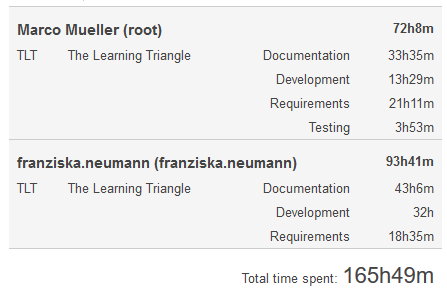
\includegraphics[scale=0.65]{bilder/TimeReport.PNG}
\caption{Time Report}
\label{TimeReport}
\end{figure}

Unterschieden wird zwischen vier Kategorien, in die Tasks unterteilt werden. \textit{Documentation} vereint dabei alle Aufgaben im Zusammenhang mit dem Schreiben der Studienarbeit, also beispielsweise das Aufsetzen eines LaTeX-Dokumentes oder der Korrekturlese. \textit{Developement} beinhaltet alle Tasks der Entwicklung, \textit{Requirements} sind nötige Vorarbeiten wie das Aneignen von Wissen. \textit{Testing} beschreibt das Testen von Anwendungen oder Ergebnissen. Diese vier Bereiche wurden so gewählt um möglichst alle Aufgabenkategorien abzudecken und dabei nicht zu viele Bereiche zu benötigen. Eine genaue Analyse mit Begründung und ein Fazit der Zeiten findet sich im Fazit in Kapitel \ref{fazitChapter}.

\section{Meilensteine und Qualitätssichernde Maßnahmen}

Ein wichtiger Bestandteil der Planung sind die Meilensteine sowie die Qualitätssichernden Maßnahmen. Meilensteine bilden dabei wichtige Zwischenschritte zur Zielerreichung. Die Qualitätssichernden Maßnahmen stellen sicher, dass diese Meilensteine auch erreicht werden. Die Planung diesbezüglich wurde in der Tabelle \ref{QSMSAnalyseBild} auf Seite \pageref{QSMSAnalyseBild} im Anhang festgehalten und jeweils zum Sprintwechsel analysiert.

Des weiteren wurde eine Meilenstein-Trend Analyse je Semester, zu sehen in Abbildungen \ref{MTA} und \ref{MTA6} auf Seite \pageref{MTA} und \pageref{MTA6} im Anhang, angelegt. Diese zeigen auf einen Blick, ob das Projekt in Verzug ist, oder ob alles in Ordnung ist. Wenn die farbigen Balken horizontal verlaufen, ist das Projekt im Zeitplan. Würde das Projekt in Verzug geraten, würden die farbigen Balken diagonal nach oben wachsen, so wie es rechts oben in der Abbildung \ref{MTA} zu sehen ist. Da es sich hier um eine Verzögerung von lediglich 3 Tagen handelt, kann gesagt werden, dass das Projekt noch im Zeitplan ist. Der unterste Meilenstein in Abbildung \ref{MTA6} wurde im Laufe des Projekts gestrichen. 

\section{Risikomanagement}
\label{riskmanagementchapter}
Ein weiterer wichtiger Bestandteil der Planung ist das Risikomanagement. Dabei geht es darum, vor Projektstart mögliche Risiken zu analysieren um ihnen im Falle eines Auftretens schnell entgegenwirken zu können. Durch Risikomanagement kann bei guter Planung das Erreichen der Projektziele abgesichert werden, sowie ein Scheitern des Projekts verhindert werden. Tritt zum Beispiel ein Problem auf, auf welches schnell reagiert werden muss, ist es vorteilhaft, wenn die Situation vorher schon bedacht wurde. Auch wenn manche Probleme nicht vollständig eliminiert werden können, so kann der Schaden doch reduziert werden.

Deshalb wurden für das Projekt folgende Problemszenarien ermittelt, deren Risikofaktor anhand Auftrittswahrscheinlichkeit und erwartetem Schaden errechnet sowie mit Gegenmaßnahmen ausgestattet. Zudem gibt es für jedes Szenario einen Verantwortlichen, welcher das Risiko im Auge behält um so möglichst frühzeitig die Gegenmaßnahmen einzuleiten. 

\paragraph{Wissensproblem - 50\% - beide}
Das größte Risiko bergen die beiden großen neuen Themengebiete AI und \textit{Educational Game}. Diese müssen für die Bearbeitung der Studienarbeit in einem gewissen Maß erarbeitet und verstanden werden. Bei schlechter Erarbeitung kann unter Umständen der Sinn des Projektes nicht erfüllt werden.

Um dem entgegen zu wirken, muss ausreichend Zeit für die Aneignung von Wissen zum Thema AI, für das Erarbeiten der Lernmethodik sowie die Durchführung eingeplant werden.

\paragraph{Klausuren - 35\% - Franziska Neumann}
Aufgrund der Erfahrung aus den letzten Jahren wird es zum Ende des Semesters oftmals stressig, da die Klausuren anstehen. Die Klausurvorbereitung nimmt dann einen großen Teil der zur Verfügung stehenden Zeit ein. Darunter kann die Studienarbeit leiden.

Deshalb sollte bei der YouTrack-Planung immer die Klausurenphase im Blick behalten werden. Große, zeitaufwendige Tasks sollten vor der stressigen Zeit erledigt werden.

\paragraph{Planung - 25\% - Marco Müller}
Ein weiteres Risiko stellt die Planung dar. Oftmals soll mehr erreicht werden als erreicht werden kann. Die unrealistische Planung kann dann aber zu Zeitproblemen führen. 

Eine Möglichkeit realistischer zu Planen stellen dabei Retrospektiven dar. In diesen wird erarbeitet, was und wie viel in welcher Zeit erledigt werden konnte. Daraufhin kann geplant werden, welche Tasks in Zukunft etwa wie viel Zeit brauchen werden.

\paragraph{Hardware - 21\% - Marco Müller}
Um ein neuronales Netz zu trainieren braucht es viel Rechenleistung. Ein Risiko ist hierbei, dass die private Rechenleistung nicht ausreicht um die Algorithmen der künstlichen Intelligenz fristgerecht zu berechnen. 

Eine Möglichkeit dieses Problem zu umgehen, ist, die \glqq Rechenleistung\grqq{} auslagern und zum Beispiel die DHBW-Computer (mit-)zu verwenden. Hierbei muss jedoch rechtzeitig ein Bedarf bei den Ansprechpartnern angemeldet werden.

\paragraph{Inkompatible Tools - 14\% - Marco Müller}
Sobald ein Projekt größer wird, werden verschiedene Tools eingesetzt. Dabei kann es passieren, dass diese nicht zusammen passen. 

Daher sollte im Vorhinein geplant werden, welche Software verwendet werden soll und geprüft werden, ob diese zusammen arbeiten. Ist dies nicht der Fall sollte nach einer alternativen Software gesucht oder ein Workaround gefunden werden.

\paragraph{Krankheit - 12\% - Franziska Neumann}
Ein weiteres Risiko besteht darin, dass ein Teammitglied krankheitsbedingt ausfällt. 

Leider kann hiergegen nicht sehr viel mehr vorbeugend unternommen werden, als darauf zu achten, ausreichend Vitamine zu essen und auf die nötige Hygiene zu achten.

\paragraph{Kommunikation - 12\% - Franziska Neumann}
Schlechte oder keine Kommunikation führt oftmals zu Missverständnissen und kann das Ziel des Projekts gefährden. Des Weiteren können Schwierigkeiten im Team ein gutes Vorankommen des Projekts verhindern.

Um dies zu verhindern sollten regelmäßige Treffen vereinbart werden und der Kontakt ständig über Email, Messenger, Telefon sowie vor Ort in der Uni gehalten werden.

\chapter{Grundlagen}

\section{Was ist \textit{The Learning Triangle} (TLT)}

Dieser Abschnitt befasst sich mit der Vorlage für dieses Projekt, The Learning Triangle. Es werden das grundlegende Prinzip sowie die wichtigsten Regeln erklärt und auch die technische Seite wird erläutert. Abschließend wird beschrieben, wie TLT im Zuge dieser Arbeit weiterverwendet wird. 

\subsection{Grundidee}

Im Rahmen des Software Engineering Kurses an der DHBW Karlsruhe sollte in Gruppen von zwei bis vier Studenten ein eigens gewähltes Projektthema erarbeitet werden. Eines der Projekte aus dem Studienjahr 2016/17 war TLT. Die Grundidee des Projektes war die Simulation des Verhaltens von Kreaturen, den namensgebenden \grqq Triangles\glqq{}. Sie sollten sich bewegen und auf ihre Umwelt reagieren, mit dem Ziel, solange wie möglich zu überleben. Das dafür nötige Wissen wurde ihnen jedoch nicht mithilfe einprogrammierter Regeln vorgegeben, sie sollten es eigenständig aufbauen. Am Allerbesten eignet sich dafür künstliche Intelligenz. 

\subsection{Regelwerk}

Zu Beginn musste ein Rahmen festgelegt werden, der die Regeln des Programms beschreibt. Dabei wird zwischen verschiedenen Regelbereichen unterschieden, den Regeln für die Triangles, den Regeln für die Oberwelt und den allgemeinen Spielregeln. Auf alle soll im Folgenden eingegangen werden.

\subsubsection{Allgemeine Regeln}

Die Allgemeinen Regeln beschreiben die Zusammenhänge der einzelnen Spielelemente. Pro Spiel existiert eine Oberwelt auf der sich eine beliebige Menge an Triangles befindet. Gesteuert werden diese Triangles nicht durch vorhandene Algorithmen, die wissen welcher Pfad der Beste ist, sondern durch eine künstliche Intelligenz, die sich dieses Wissen erst erarbeiten muss. 

Das Spiel startet mit der Erstellung einer Oberwelt, gefolgt vom eigentlichen Spielablauf mit dem Abschließen des Spiels durch den Tod aller Triangles. Ein Siegkriterium ist nicht vorhanden. Wie die Oberwelt erstellt wird kann in \ref{subsubsec_oberweltregeln} nachgelesen werden. Der Spielablauf an sich erfolgt in kurzen Zyklen. In jedem Zyklus bewegt sich jedes Triangle ein Feld in eine von der KI bestimmten Richtung. Die Feldaktionen werden ausgeführt und ein neuer Zyklus beginnt.

Das durch die allgemeinen Regeln festgelegte Ziel ist eine möglichst lange Lebenserhaltung aller Triangles. Da ein Algorithmus mit dieser Aussage wenig anfangen kann und es zu ungewollten Lösungen kommen kann, muss das Ziel greifbarer ausgedrückt werden. Deshalb lautet das der AI mitgeteilte Ziel, so viel Strecke wie möglich zurückzulegen, was sich nur durch eine lange Lebensspanne aller Triangles realisieren lässt. Bereits in der Vergangenheit gegangene Wege erhöhen den Distanzwert erneut, sodass es keinen Maximalwert gibt.

\subsubsection{Oberwelt-Regeln}
\label{subsubsec_oberweltregeln}
Diese Regeln beschreiben, wie die Oberwelt erstellt wird und welche Vorgaben dabei beachtet werden müssen. Die wichtigste Eigenschaft der Map ist die beliebig große quadratische Oberwelt, bestehend aus einzelnen, ebenfalls quadratischen Feldern. Diese Felder besitzen verschiedene Eigenschaften welche in Tabelle \ref{tbl_fields} näher erläutert werden. \\

\begin{center}
\label{tbl_fields}
\begin{tabular}{ | p{1.5cm} |p{3cm} | p{8.5cm}| c r r }
\hline
Bild & Feld-Typ & Eigenschaft \\
\hline

\includegraphics[scale=0.6]{bilder/Style-Classic_Normal_Field.png} & Normal-Field & Das Standard-Feld, welches keine Effekte auf das Triangle wirken lässt. Es kann betreten und verlassen werden. \\ 
\hline

\includegraphics[scale=0.6]{bilder/Style-Classic_Wall_Field.png} & Wall-Field & Auf der Oberwelt gibt es nicht passierbare Felder, die das Triangle nicht überqueren kann. Diese Felder sind Wall-Fields. \\ 
\hline

\includegraphics[scale=0.6]{bilder/Style-Classic_Energy_Field.png} & Energy-Field & Das Triangle besitzt eine begrenzte Menge Energie. Diese wird um eine festgelegte Menge erhöht, sollte dieses Feld betreten werden. Dieser Vorgang ist einmalig, das Energiefeld verliert seine Eigenschaften bei Kontakt. Dies verhindert, das die AI Triangles einfach zwischen Energie-Feldern und anderen Feldern hin- und herbewegt, da sie ohne diese Regel dafür unbegrenzt Energie und Strecke erhalten würde.\\
\hline

\includegraphics[scale=0.6]{bilder/Style-Classic_Poison_Field.png} & Poison-Field & Bei jedem Schritt braucht ein Triangle Energie. Das berühren dieses Feldes erhöht die nötige Menge Energie einer Triangle-Bewegung für einige zukünftige Zyklen des Spielablaufs. \\ 
\hline

\includegraphics[scale=0.6]{bilder/Style-Classic_Death_Field.png} & Death-Field & Bei Kontakt mit diesem Feld verliert das Triangle seine ganze Energie und stirbt. \\ 
\hline
\end{tabular}
\end{center}

Die Oberwelt kann über zwei verschiedene Arten erstellt werden. Es ist möglich, eine vorhandene, korrekt formatierte Datei einzulesen und als Map zu verwenden, die Oberwelt kann aber auch zufällig generiert werden. Dabei lässt sich einstellen, wie hoch die Wahrscheinlichkeit für die einzelnen Felder sein soll. Jede generierte Oberwelt lässt sich für die zukünftige Verwendung wieder in eine Datei speichern. Mithilfe der Implementierung eines Mapbuilders lassen sich diese Dateien bearbeiten.

\begin{figure}
\centering
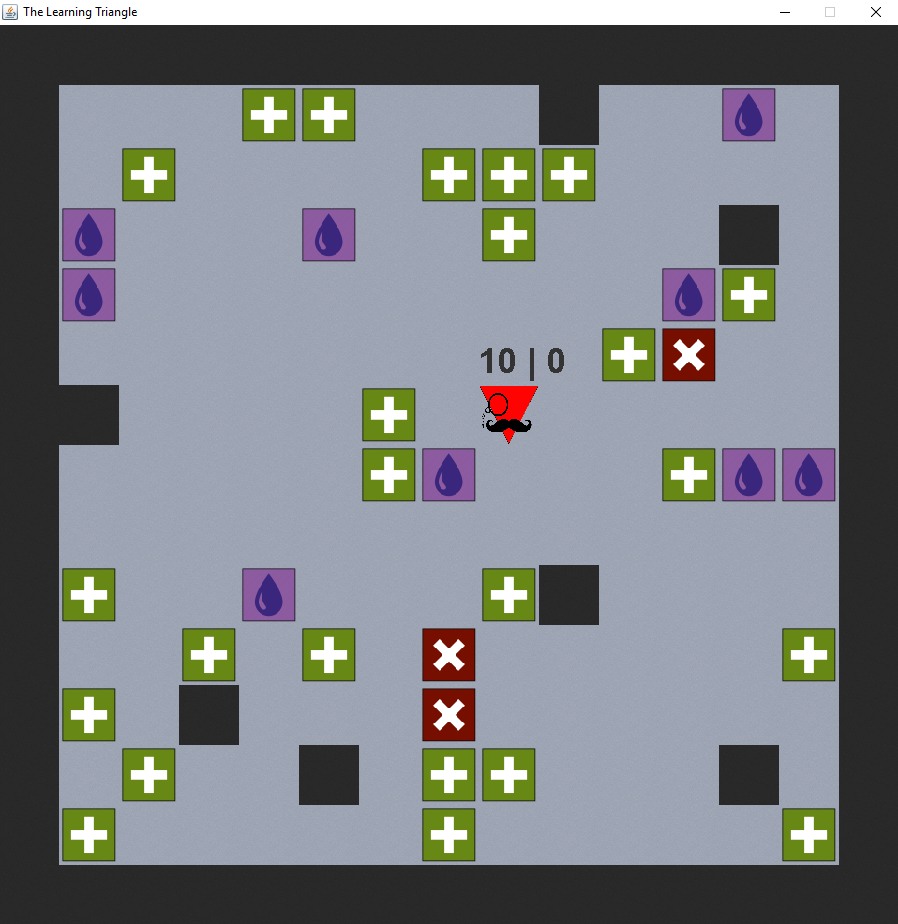
\includegraphics[scale=0.5]{bilder/TLT_Game.PNG}
\caption{Beispiel für eine zufällig erstellte Oberwelt}
\label{BeispielMapTLT}
\end{figure}


\subsubsection{Triangle-Regeln}

Für jede Instanz eines Triangle gelten Regeln. Diese beschreiben unter anderem auch die Fähigkeiten eines Triangles. Grundlegend gesehen ist die Implementierung eines Triangles eine sehr vereinfachte Variante eines kleinen Lebewesens. Es besitzt eine festgelegte Menge an Energie, welche es bei Bewegung verbraucht. Ist alle Energie verbraucht, stirbt das Triangle. Das Ziel von TLT war es, solange wie möglich zu überleben. Zu diesem Zweck muss das Triangle ausreichend oft Energie-Felder betreten. Um diese zu finden besitzt jedes Triangle ein Sichtfeld, bestehend aus allen Felder um die aktuelle Position herum verteilt. Der Radius ist dabei festgelegt. Die Bewegung des Triangles erfolgt in vier mögliche Richtungen: Norden, Süden, Osten und Westen. Die Entscheidung in welche Richtung gegangen werden soll trifft das Triangle nicht selbst. Diese Aufgabe wird von dem implementierten AI-Algorithmus getroffen.

\subsection{Bisherige Technische Seite des Projektes TLT}
\label{bisherigeTechnikTLT}

Technisch basiert TLT auf Java. Es existieren drei verschiedene Schichten im bisherigen Projekt: Die Anwendungsoberfläche, in der nachvollzogen werden kann was gelernt wurde und was dann mit den Triangles passiert, wird dieses Wissen angewendet. Darunter liegt das Regelwerk, welches die beschriebenen Regeln implementiert und gewährleistet, dass keine unerwarteten Dinge passieren. Hier werden auch alle Parameter konfiguriert. Den Abschluss bildet die Implementierung des \textit{Deep Learning} Algorithmus, im bisherigen Projekt war das die Bibliothek DeepLearning4Java. Dabei wurde ein neuronales Netzwerk aufgebaut welches als Eingabe das Sichtfeld eines Triangles erhält und als Ausgabe eine Richtung vorhersagt. Verwendet wurde dafür \textit{Reinforcement Learning} (siehe Kapitel \ref{machinelearning_ansaetze}), der Algorithmus wurde also fortlaufend mit einer Fitness bewertet. Perfekt ausgereift war die Implementierung der AI noch nicht, an vielen Stellen hätte noch gearbeitet werden können.

\subsection{Weiterverwendung des Projektes TLT}

Im Zuge dieses Projektes soll TLT zu einem \textit{Educational Game} werden. Verschiedene Begriffe und Algorithmen sollen erklärt werden. Damit das gut funktioniert ist eine häufige Neuimplementation vieler bereits entwickelter Bestandteile in leicht abgeänderter Form nötig. Das dieser Prozess möglichst wenig Aufwand verursacht und gut funktioniert muss eine klare Trennung zwischen den einzelnen technischen Bereichen geschaffen werden. TLT muss möglichst modular und austauschbar sein. Die bisher vorhandene Struktur ist für dieses Ziel von großem Nutzen, auch in Zukunft sollen die drei Schichten beibehalten werden. Ergänzt wird TLT durch eine weitere wichtige Schicht, in der die Daten gespeichert werden. Damit sind vor allem Erklärungstexte und Spielparameter gemeint.

Die Flexibilität der Regeln und Parameter ist eine große Stärke von TLT. Dies ermöglicht die fast uneingeschränkte Weiterverwendung des Projektes im Zuge der Erstellung eines \textit{Educational Game}. So werden einige der im Kommenden beschriebenen Regeln für spezifische Aufgaben angepasst oder aufgehoben, wieder andere werden dafür ins Regelwerk aufgenommen. Die Grundstruktur bleibt dabei bestehen.

\section{Was ist ein Educational Game}

\subsection{Definition}

\textit{Educational Game}, Lernspiel oder didaktisches Spiel wie die Spielwissenschaft solche Spiele bezeichnet, es gibt viele Begriffe, die jedoch ein und das selbe bezeichnen. \\

\begin{addmargin}[25pt]{0pt} 
\glqq An \textit{Educational Game} is a game designed to teach humans about a specific subject and to teach them a skill.\grqq \cite{F_DefinitionEducationalGame_3.2}
\end{addmargin}

\ \\ Ein \textit{Educational Game} ist demnach ein Spiel, das dazu gedacht ist, Menschen über ein bestimmtes Thema aufzuklären und ihnen eine Fertigkeit beizubringen. Das Ziel ist es, das Wissen auf eine Art und Weise zu vermitteln welche Spaß macht. Dabei ist die Form des \textit{Educational Game} völlig frei wählbar. Es kann sowohl als Brettspiel vorliegen, als auch ein Kartenspiel oder Computerspiel sein. 

Allerdings ist eine genaue Abgrenzung zwischen einem normalen Spiel und einem \textit{Educational Game} oftmals nicht einfach. Denn auch ein normales Spiel vermittelt auf irgendeine Art und Weise Wissen und Fertigkeiten. Diese Art von lernen wird auch \glqq Inzidentelles Lernen\grqq{} genannt. \glqq Beim inzidentellen Lernen handelt es sich um einen Vorgang, bei dem Informationen nebenbei (unabsichtlich) aufgenommen werden. Das bedeutet, wir lernen viele Inhalte, ohne dass eine Lernabsicht vorliegt. Der Anteil der unabsichtlichen Lernprozesse ist mindestens so groß wie der Anteil jener Lernprozesse, bei denen es eine Lernabsicht gibt. \grqq ~\cite{F_InzidentellesLernen_3.2} 

\subsection{Elemente eines Educational Game}
Die große Frage ist: Was machen \textit{Educational Games} anders? Dafür ist es hilfreich einen Blick in deren Vergangenheit zu werfen. Zunächst gab es einfache Vokabeltrainer, die über ein Belohnungssystem den Lernenden motivierten. Eine richtige Eingabe gab Punkte, falsche Angaben wurden über Punktabzug bestraft. Die nächste Stufe stellten interaktive Enzyklopädien dar. Der Spieler konnte darin seine Umgebung wie eine Art Museum erkunden und so die Lerninhalte selbständig erarbeiten. Inzwischen werden durch \textit{Educational Games} Mikrowelten generiert, in denen der Lernstoff spielerisch präsentiert wird. Meist wird dabei eine interaktive Geschichte erzählt. 

Wo liegen nun also die Unterschiede zum normalen Frontal-Unterricht? Als erstes sei das Belohnungssystem zu erwähnen. Das gibt es in der Form an Schulen oder Universitäten nicht. Dort wird eher ein Fehlerbestrafungssystem praktiziert. Das heißt, der Schüler lernt oftmals bloß aus Angst vor den Konsequenzen den Stoff. In der Psychologie wird diese Art von Motivation auch extrinsisch genannt. Das Problem dieser Form von Motivation ist, dass sie nur bestehen bleibt, solange die Leistung auch überprüft wird. \textit{Educational Games} hingegen setzen auf die intrinsische Motivation. Sie kommt im Gegensatz zur extrinsischen Motivation nicht von außen, sondern aus dem Innern. Das heißt die Aufgaben, welche erledigt werden müssen entsprechen den eigenen Wünschen. Vereinfacht gesagt wird das Spielen des \textit{Educational Games} zum eigenen Wunsch des Spielenden, da durch das Belohnungssystem ein Anreiz geschaffen wird, weiter zu spielen und somit auch zu lernen. Ein weiterer Vorteil den \textit{Educational Games} bieten, liegt im \glqq Trial-and-Error \grqq Prinzip. Der Spielende kann Dinge ausprobieren und aus den Fehlern lernen. Da Fehler an Schulen oftmals mit negativen Gefühlen und Konsequenzen verbunden werden, fällt der Effekt des Sprichworts \glqq aus Fehlern lernen \grqq oftmals weg. Der Vorteil den hier \textit{Educational Games} mitbringen liegt darin, dass durch das Fehlen von Erwartungen an einen direkten Nutzen, Fehler nicht negativ ins Gewicht fallen \cite{F_VorteileEducationalGames_3.2.2}

Was braucht es, damit ein \textit{Educational Game} erfolgreich ist? Zunächst sollte das Spielen Spaß machen und zum weiterspielen anregen. Dies kann zum Beispiel in Form einer interaktiven Geschichte erreicht werden. Ein positiver Nebeneffekt einer Geschichte ist, dass der Lernaktivität ein Sinn gegeben wird. Jedoch muss darauf geachtet werden, dass das Spielziel dem Lernziel entsprechen sollte. Das heißt, um ein Level weiter zu kommen, muss der vermittelte Lerninhalt verstanden sein. Ein weiterer Bestandteil, welcher ein \textit{Educational Game} erfolgreich machen kann ist die Möglichkeit der sozialen Interaktion. Das kann zum Beispiel dadurch erreicht werden, dass Klassenkameraden zusammen wirken müssen, um eine Aufgabe zu lösen, oder in einem anderen Spielmodi gegeneinander antreten können, um eine Rangliste untereinander auszuspielen. \cite{ F_erfolgreicheEducationalGames_3.2}

\subsection{Beispiele}
In \textit{Educational Games} wird in erster Linie Wissen vermittelt.Die Tabelle \ref{tbl_educationalGames} enthält einige Beispiele und was das jeweilige \textit{Educational Game} vermitteln möchte.\newline

\begin{center}
\label{tbl_educationalGames}
\begin{tabular}{ |p{3cm} | p{10cm}| c r }
\hline
Spiel & Lerninhalte \\
\hline
Boggle, Galgenmännchen & Um zu gewinnen muss jeweils ein deutsches Wort beziehungsweise so viele deutsche Wörter wie möglich gefunden werden. Dabei kann die Rechtschreibung geübt und der Wortschatz erweitert werden. Diese Spiele eignen sich auch dafür, Fremdsprachen zu lernen. \\  
\hline
Stadt-Land-Fluss & In diesem Spiel können die geografischen Kenntnisse der Spieler erweitert werden. \\
\hline
Schiffe versenken & Durch Schiffe versenken lernt der Spieler den Umgang mit Koordinatensystemen.   \\ 
\hline
Brain It On! & In diesem Smartphone Spiel müssen verschiedene Rätsel durch zeichnen von Formen gelöst werden. Dabei muss der Spieler die Gesetze der Physik, wie zum Beispiel die Schwerkraft beachten um das jeweilige Ziel zu erreichen. \\ 
\hline
\end{tabular} 
\end{center} 

Unter den Begriff \textit{Educational Game} fallen auch Spiele, welche die sozialen Fertigkeiten des Spielenden erhöhen. Eine Kombination aus der Vermittlung von Wissen und sozialen Kompetenzen gibt es natürlich auch. Ein Beispiel hierfür ist das Waldschattenspiel. In diesem Brettspiel müssen die Spieler gemeinsam gegen das Licht in Form eines Teelichts spielen. Das Spiel wird im Dunklen gespielt, damit der Unterschied zwischen Licht und Schatten besser zu erkennen ist. Auf dem Spielbrett gibt es verschiedene Wege und einige verteilte 3D Tannenbäume hinter denen sich Spielfiguren vor dem Licht verbergen können. Ziel des Spiels ist ein gemeinsames Treffen im Schatten eines Tannenbaumes. Gerät eine Spielfigur ins Licht müssen die Mitspieler versuchen, durch Bewegen des Lichts, die Figur wieder zu befreien. Das Waldschattenspiel vermittelt also nicht nur den Wissenschaftlichen Aspekt von Licht und Schatten sondern fördert die Kooperation mit anderen. \cite{F_Lernspiel_3.2}

\section{Was ist AI}

In diesem Abschnitt werden die wichtigsten Begriffe rund um \textit{Artificial Intelligence} erklärt. Dabei ist jedoch eine grundlegende wichtige Annahme wichtig. Durch den neuen Aufschwung von Machine Learning werden viele bereits seit vielen Jahren existierende Methodiken und Begriffe von vielen Seiten neu betrachtet und es gibt deshalb keine klare Definition für jeden einzelnen Fachbegriff. Stattdessen gibt es Meinung, wie genau Begriffe zu definieren sind, die aber immer wieder validiert und/oder angepasst werden. Das erschwert die Situation, klare Aussagen zu treffen. Die nachfolgenden Erklärungen sind deshalb unter Anbetracht des aktuellen Datums und der Freiheit, auch anders definiert sein zu können zu lesen. Beruhigend ist, das keine großen Unterschiede zwischen den Auslegungen existieren, sondern nur kleine Differenzen. Keine der Definitionen ist deswegen grundlegend falsch oder anders.

\subsection{Definitionen} 

Zunächst soll der Begriff AI genauer definiert werden. \\

\begin{addmargin}[25pt]{0pt} 
\glqq Artificial intelligence (AI) is an area of computer science that emphasizes the creation of intelligent machines that work and react like humans. Some of the activities computers with artificial intelligence are designed for include: Speech recognition, Learning, Planning, Problem solving\grqq \cite{F_AIDfinition_3.3.1}
\end{addmargin}

\ \\ AI ist ein Bereich der Informatik, in dem an künstlichen Intelligenzen geforscht wird. Allerdings ist das Forschungsgebiet keinesfalls geschlossen. Viele andere Wissenschaften wirken bei der Entwicklung mit. Es geht darum, Systeme zu entwickeln, die Aufgaben erledigen können, bei denen normalerweise menschliches Denken benötigt wird. Dazu gehören zum Beispiel Spracherkennung, Bilderkennung, Übersetzungen, Entscheidungen anhand mehrerer Faktoren richtig treffen und neue Dinge zu lernen. Entgegen der weit verbreiteten Vorstellungen muss eine AI nicht unbedingt die Fähigkeit haben, dazuzulernen. Viele Systeme klassifizieren \glqq nur\grqq{} die vorliegenden Daten, oder extrahieren Wissen daraus. Ein ebenfalls weit verbreiteter Irrtum ist, dass eine AI intelligent ist, jedoch wird mittels Mathematik und Informatik lediglich intelligentes Verhalten simuliert. Von der Schaffung eines Bewusstseins ist die Forschung noch unabsehbar weit entfernt.

\paragraph{Starke künstliche Intelligenz} Die Schaffung eines Bewusstseins wird durch den Begriff starke künstliche Intelligenz beschrieben. Sie beschäftigt sich damit, menschliches Denken zu mechanisieren, damit eine Maschine wie ein Mensch reagieren kann. Wie oben schon beschrieben, ist dieser Bereich von AI eher eine Vision. Es ist unklar, ob es realistisch ist, die Ziele in naher Zukunft zu erreichen.

\paragraph{Schwache künstliche Intelligenz}
Die schwache künstliche Intelligenz hingegen hat es sich zum Ziel gemacht, konkrete Anwendungsprobleme des menschlichen Denkens zu meistern und den Menschen \glqq beim Denken\grqq{} zu unterstützen. Da kaum Begrenzungen an Einsatzgebieten vorhanden sind, wurden schon viele kleine und große Erfolge in verschiedenen Bereichen gefeiert.

\paragraph{Data Sets}
Damit die Algorithmen ordentlich arbeiten können ist es von enormer Wichtigkeit, die richtigen Daten im richtigen Format vorliegen zu haben. Diese Beziehung gilt natürlich auch umgekehrt. Der Algorithmus muss umso besser werden, je größer die Unsicherheiten bzw. problematischen Informationen in den Daten sind. ~\cite{F_KI_3.3.1}

\paragraph{Der Turing-Test}
Der Turing-Test ist ein von Alan Turing entwickelter Test, welcher ein Maß dafür gibt, wie gut bzw. ob eine Maschine die Intelligenz eines Menschen gleichwertig simuliert. Seit 1991 existiert ein Preis für denjenigen, dessen Maschine den Test besteht. Bisher hat das aber noch niemand geschafft. Um den Test zu bestehen, darf die Testperson nicht unterscheiden können, ob es sich bei seinem Gesprächspartner an einem Terminal um einen echten Menschen oder eine Maschine handelt. Die Person stellt dabei beliebige Fragen, ohne zu wissen, wer ihm antwortet. Kann die Person am Ende Mensch und Maschine nicht unterscheiden, hat die Maschine den Test bestanden. ~\cite{F_TuringTest_3.3.1}

\subsection{Machine Learning}

\textit{Machine Learning} ist ein Teilgebiet im Bereich der künstliche Intelligenz. Es beschreibt alle Algorithmen, die nicht auf fixes Wissen beschränkt sind, sondern durch mathematische Formeln in der Lage sind, ihr Wissen zu erweitern und sich auf bestimmte Probleme anzupassen. Das genaue Verständnis soll auf den kommenden Seiten klar werden.

\subsubsection{Ansätze}
\label{machinelearning_ansaetze}

Die Bezeichnung Ansätze ist ein inoffizieller Begriff für die Art und Weise des Lernens. Generell lassen sich fast alle Algorithmen in einen von drei Bereichen einteilen. Diese drei Bereiche sollen im Kommenden genauer erklärt werden.

\paragraph{Supervised Learning}
Der Begriff \textit{Supervised Learning}, zu deutsch überwachtes Lernen, beschreibt ein Ansatz beim Lösen von Lern-Problemen. Die Idee von \textit{Supervised Learning} ist, einen AI-Algorithmus mithilfe eines bekannten Ergebnisses lernen zu lassen. Genauer gesagt ist dem Algorithmus bereits zu Beginn bekannt, welche Ergebnisse oder Klassen für den Anwendungsfall zu erwarten sind. Realisiert wird dies indem der Algorithmus zu Beginn mit einer Datengrundlage ausgestattet wird anhand derer er lernen kann. Diese zeigt dem Algorithmus zu welchem Ergebnis er kommen hätte müssen hätte er mit den Daten gearbeitet und kann dieses Wissen bei neuen Situationen anwenden. Am Beispiel der Bilderkennung ausgedrückt hat ein Algorithmus die Vorgabe, dass ein Bild entweder einen Hund oder eine Katze zeigt. Neue einzuordnende Bilder werden jetzt den bekannten Klassen zugeordnet.\cite{M_DL4J_Many}

\paragraph{Unsupervised Learning}
Ganz im Gegensatz zu \textit{Supervised Learning} steht \textit{Unsupervised Learning}, zu deutsch unüberwachtes Lernen. In diesem Konzept hat ein AI-Algorithmus keine Ergebnisse oder Ziele an denen er erkennen kann wie mit neuen Daten umgegangen werden soll. Jedes Ergebnis muss selbst vom Algorithmus herauskristallisiert werden. Häufig wird dabei \textit{Clustering} verwendet, näheres dazu siehe in Kapitel \ref{MLTechniken}. Dabei werden Lösungsgruppen gefunden. Im Fall der Bilderkennung kann ein Algorithmus somit nicht sagen das er Bilder mit Hunden und Katzen vor sich hat, er ist aber in der Lage eine klare Grenze zwischen verschiedenen Bilder zu ziehen und sie in unterschiedliche Merkmalsgruppen einzuteilen, da ein Hund nicht wie eine Katze aussieht.\cite{M_DL4J_Many}

\paragraph{Reinforcement Learning}
\textit{Reinforcement Learning}, der dritte der drei Bereiche und zu deutsch bestärkendes Lernen, wählt einen Ansatz bei dem ein Wert errechnet wird, der verbessert werden soll. Dieser Wert wird auch Fitness genannt. Bei jedem Durchlauf wird als Ergebnis eine Zahl ausgegeben, anhand derer der Algorithmus erkennen kann wie gut er war. Was dabei als gut zu bezeichnen ist, ist eine Frage der Kalibrierung, im Normalfall steht eine höhere Fitness aber für ein besseres Ergebnis. Ziel des Algorithmus ist es die Fitness zu verbessern um als Folge den gesamten Lernprozess zu optimieren. \cite{M_Reinforcement_3.3.2.1}

\subsubsection{Neural Network}
\paragraph{Die Geschichte} Die Idee zu neuronalen Netzen kam das erste Mal in den 1940er Jahren auf. Der Neuropsychologe und Kybernetiker Warren McCulloch entwickelte zusammen mit Walter Pitts, ebenfalls Psychologe spezialisiert auf die Kognition, das Modell des McCulloch-Pitts-Neurons. Er forschte dabei über die Funktionsweise des menschlichen Gehirns und entwickelte dabei die uns heute bekannte Auffassung über neuronale Netze. Die beiden Wissenschaftler konnten beweisen, dass mit einem endlichen Netz solcher sogenannten Neuronen turing-berechenbare Probleme gelöst werden können. Allerdings fehlte damals ein leistungsfähiger Computer, weswegen die Idee der Neuronalen Netze bis in die Mitte der 80er in den Hintergrund geriet.

Der aufkommende Konnektionismus orientierte sich wieder an dem menschlichen Gehirn als Vorbild. Die Grundidee bestand daraus, dass das Verarbeiten einer Information in vielen simplen einheitlichen Verarbeitungselementen parallel erfolgt. Die Forscher setzten also die bereits entwickelten Neuronen in einem Netz ein und brachten dem System anhand von Beispielsätzen das Sprechen bei. Das funktionierte bis zu einem gewissen Maß sehr gut, denn die Netze lernten gut und schnell. Allerdings waren die Computer zu der Zeit immer noch nicht leistungsfähig genug. Zudem fehlte es an genügend strukturierten Trainingsdaten.

Seit 2010 kommen die Neuronalen Netze nun richtig zur Geltung. Ursachen dafür sind die nun vorhandenen ausreichenden Rechenleistungen und die zunehmende Verfügbarkeit an strukturierten Daten, mit denen die Algorithmen trainiert werden können. Weitere Aspekte sind die Weiterentwicklung der Neuronalen Netze, verbesserte Algorithmen und vor allem eine Variante der neuronalen Netze: \textit{Deep Learning}. ~\cite{F_neuronaleNetze_3.3.2.2} In Abschnitt (Deep NN) wird \textit{Deep Learning} genauer betrachtet.

\paragraph{Elemente eines neuronalen Netzwerks}
Jedes neuronale Netz besteht aus vielen Neuronen oder auch Knoten, welche untereinander auf eine bestimmte Art und Weise vernetzt sind. Die Art der Vernetzung, auch Topologie genannt ist abhängig von dem zu lösenden Problem und sollte gut durchdacht sein. Das Netz kann in verschiedene Layer aufgeteilt werden: Input, Hidden und Output Layer. Dabei besteht jedes Layer aus einer beliebigen Anzahl von Knoten. Jeder Input kann gewichtet werden und jeder Output kann durch einen Optimierungsalgorithmus optimiert werden. ~\cite{M_DL4J_Many}

\paragraph{Convolutional NN}
\textit{Convolutional Neural Networks} finden ihre wichtigste Anwendung in der Bildklassifizierung. Als Input wird dabei eine zweidimensionale Matrix, meistens die Pixel eines Bildes, verwendet. Im Anschluss wird ein kleineres Matrixfeld mit eigenen Werten über das Input-Feld bewegt. Die Werte des kleinen Feldes werden dabei selbst erlernt. Die Berechnung der Output-Matrix erinnert dabei an das Skalarprodukt, verwendet werden alle Werte aus beiden Matrizen im Bereich der Überschneidung, deren Ergebnisse wiederum miteinander verrechnet werden. Das Ergebnis dieser Berechnung wird dann in der Output-Matrix an die passende Stelle geschrieben. Das Prinzip ist auch unter dem Begriff \textit{Faltung} aus der Bildverarbeitung bekannt. \cite{M_CNN_3.2.2.2}

\newpage

\paragraph{Deep NN}
\textit{Deep Neural Networks} werden beim oben genannten \textit{Deep Learning} verwendet. Der Unterschied zu einem gewöhnlichen neuronalen Netzes besteht darin, dass es über mehrere Hidden Layer verfügt. Das Ziel des Trainings ist es, einen möglichst geringen Fehler im Output zu erreichen. Ein Training durchläuft normalerweise folgende Phasen:
\begin{itemize}
\item Netz durchlaufen
\item Vermutung aussprechen
\item Fehlermessung
\item Aktualisierung der Gewichte
\item Weiter bei Punkt 1
\end{itemize}

\textit{Deep Learning} wird häufig zur statistischen Datenerkennung verwendet und eignet sich aufgrund der großen Lernfähigkeit sehr gut für eine große Menge an \glqq unlabeled Data\grqq{}. Das ist auch der Grund, warum \textit{Deep Learning} in letzter Zeit einen so großen Aufschwung erlebt. Denn der größte Teil an Daten liegt unkategorisiert vor. Unter anderem mit Hilfe von \textit{Deep Learning} konnte im Januar 2016 der Weltmeister im Spiel Go durch eine Maschine besiegt werden. Doch nicht nur beim Go spielen dominiert \textit{Deep Learning}, das Spracherkennungsmodul von Apple's Siri basiert ebenfalls auf diesem Verfahren. ~\cite{F_DeepLearning_3.3.2.2}

\subsubsection{Techniken}
\label{MLTechniken}

Algorithmen lassen sich nicht nur nach ihren Ansätzen unterteilen, sondern auch, welches Vorgehen sie bei der Durchführung verfolgen. Unterschieden wird zwischen mehreren Techniken, von denen hier die wichtigsten kurz erläutert werden sollen.

\paragraph{Classification}
Die Klassifizierung beschreibt eine eindeutige Zuordnung eines Objektes zu einer Klasse. Diese Technik wird häufig im Zusammenhang mit \textit{supervised learning} verwendet. So ist es ein übliches Beispiel für Klassifizierung, festzustellen, was auf einem Bild angezeigt wird. Als Lerngrundlage wird einem AI-Algorithmus eine möglichst große, aussagekräftige Datengrundlage gegeben, die bereits die Aufgabe erfüllt. In diesem Beispiel können das 1000 Bilder sein, die unter dem Aspekt eingeteilt wurden, was auf Ihnen zu sehen ist (Hund, Katze, Apfel). Der Algorithmus kann anhand dieser Grundlage lernen und verstehen, wieso die Klassifizierung so vorgenommen wurde. Dabei achtet er auf Gemeinsamkeiten zweier gleich eingeordneter Bilder und auf Unterschiede der Bilder in unterschiedlichen Klassen. Anschließend sollte er in der Lage sein, eine eigene, möglichst genaue Einteilung bei neuen Bilder vorzunehmen. \cite{M_DL4J_Many}

\paragraph{Clustering}
\textit{Clustering} ist im Gegensatz zu \textit{Classification} eine Technik im Bereich \textit{unsupervised learning}. Im Rahmen des Beispiels wird ein Algorithmus zu Beginn nicht mit einer Datengrundlage ausgestattet, sondern wird sozusagen blind Bilder einteilen. Dabei wird er die Unterschiede zwischen Bildern erkennen und Ähnlichkeiten feststellen. So werden auch bei dieser Methode als Ergebnis mehrere Klassen, hier besser Gruppen genannt, gefunden. Diese werden je nach Granularität und Einstellung ebenfalls auf Hunde, Katzen und Äpfel getrennt sein, auch wenn der Algorithmus nicht weiß, dass sie als solche bezeichnet werden. Im Grunde genommen bedeutet \textit{Clustering} also nichts anderes als die Einteilung von Dingen nach Merkmalen, ohne dass vorher eine Datengrundlage gegeben ist. \cite{M_DL4J_Many}

\paragraph{Regression}
Die Regression, welche auch schon in der Mathematik Anwendung findet, spielt im Bereich des \textit{supervised Learning} eine Rolle. Im Normalfall wird dabei nur mit Zahlen gearbeitet, welche bestimmte Parameter darstellen. Diese Parameter lassen sich dazu verwenden, das Objekt an bekannte Werte anzunähern und einen Ergebniswert zu bestimmen. Ein konkreter Anwendungsfall für Regression ist die Wertbestimmung eines Autos anhand von Faktoren wie Alter und Kilometerstand des Wagens.

\subsection{Evolutionary Algorithms}
Evolutionäre Algorithmen finden ihren Ursprung in der Natur. Die Evolution hat zum Ziel, jedes Lebewesen so anzupassen, dass es in seiner Umgebung am besten zurecht kommt. Die Optimierung funktioniert dabei über die Fortpflanzung, da meist die Lebewesen am längsten überleben, die die besten Eigenschaften für die aktuelle Situation besitzen. Durch das Mischen und Vererben dieser Eigenschaften kann die Evolution ein Lebewesen in wenigen Generationen auf den Durchschnitt gesehen länger und besser überleben lassen. Dieses Vorgehen wird durch evolutionäre Algorithmen in die Technik übernommen. Dort gilt es ebenfalls oft, eine optimale Lösung zu finden. Verwendet werden dafür die selben Ideen, die sich bereits in der Natur wiederfinden lassen. Zu Beginn werden die Lösungen selektiert, bevor diese ausgewählten Lösungen untereinander neu kombiniert werden. Ohne einen gewissen Einfluss an kontrolliertem Zufall wird es jedoch, wie in der Natur auch, weniger gut funktionieren einfach erneut zu selektieren. Deshalb muss zuerst eine Mutation einiger Lösungen durchgeführt werden. Die selektierten, neu aufgestellten Lösungen werden nun mit einem Fitness-Wert versehen, bevor mithilfe von dieser der Prozess von vorne beginnt und eine erneute Selektion durchgeführt wird.

\subsection{Natural Language Processing}
NLP beschreibt ein großes Teilgebiet des \textit{Machine Learning}, die Sprachverarbeitung. Das Ziel ist eine gleichwertige Kommunikation zwischen Mensch und Maschine. Durch Text- und Stimmerkennung wurden bereits große Meilensteine im Bereich NLP erreicht, es gibt bereits Algorithmen die den höheren Sinn aneinander gehängter Worte erkennen können, selbst wenn dieser Sinn unterschiedlich ausgedrückt wird. Trotzdem gibt es noch viele Forschungsmöglichkeiten, da eine perfekte Kommunikation aktuell noch nicht gewährleistet werden kann.

\subsection{Einsatzgebiete}

Für AI gibt es viele verschiedene Einsatzgebiete. Im diesem Absatz sollen die drei Einsatzgebiete Big Data, Data-Mining und Robotik genauer betrachtet werden.

\subsubsection{Big Data}
\label{bigD}
\paragraph{Definition}
Big Data stellt keine neue Art von Daten dar, sondern vielmehr charakterisiert es, wie Daten heute immer häufiger auftreten. Um die Daten zu Charakterisieren wird oftmals das 4 V Modell von IBM verwendet.~\cite{F_BigData_3.3.5.1} Folgende Tabelle zeigt die \textit{4 V's} und ihre Bedeutung.

\begin{center}
\label{tbl_bigdata}
\begin{tabular}{ |p{1.5cm} |p{3cm} | p{8.5cm}| c r }
\hline
V & Bedeutung &  Beschreibung\\
\hline
Volume & Menge der Daten &  Im Jahr 2016 umfasste das Weltweite Datenvolumen 16,1 Zettabyte (1 Zettabyte = 1 Mrd. TB). Für 2025 wird eine Verzehnfachung erwartet\\  
\hline
Variety & Datenvielfalt & Die Daten liegen in vielen verschiedenen Formaten wie zum Beispiel Mediendateien, Textdateien, etc. vor. Dabei ist der große Anteil der Daten unstrukturiert. \\
\hline
Velocity & Geschwindigkeit & Der Zugriff auf die Daten muss größtenteils in Echtzeit erfolgen, damit eine Auswertung sinnvoll ist. Hierfür braucht es gute Algorithmen sowie die entsprechende Rechenpower. \\ 
\hline
Veracity & Aussagekraft & Das letzte der vier V steht für die Vertrauenswürdigkeit der Daten. Das Prinzip "Garbage In- Garbage Out", welches in dem Zusammenhang oftmals erwähnt wird besagt, dass nur wenn gute Daten durch einen guten Algorithmus analysiert werden, auch gute Ergebnisse erwartet werden können. Sobald der Algorithmus schlecht ist, ist der Output so gut wie unbrauchbar. \\
\hline
\end{tabular}
\end{center}

\paragraph{Zusammenhang mit AI}
Um die große Menge an Daten Effizient auswerten zu können, werden oftmals künstliche Intelligenzen eingesetzt. Die verschiedenen Modelle können die große Datenflut in der gegebenen Zeit besser bewältigen als der Mensch. Allerdings ist es unverzichtbar, wie das vierte V zeigt, auf ein gutes Model zu bauen. Big Data stellt also ein großes Einsatzgebiet für AI dar.

\subsubsection{Data-Mining}
Unter Data Mining wird die systematische Anwendung statistischer Methoden und Verfahren aus dem Bereich AI auf einen vorliegenden Datenbestand verstanden. Das Ziel von Data Mining ist es, neue Querverbindungen, Trends und relevante Zusammenhänge in den Daten zu erkennen und diese zu extrahieren. Data Mining und Big Data werden oft im selben Kontext benutzt. Allerdings bedeuten sie nicht das gleiche, wie fälschlicherweise oft angenommen. Big Data bezeichnet die Analyse großer Datenmengen aus vielfältigen Quellen in hoher Geschwindigkeit. Wie in Kapitel \ref{bigD} beschrieben ist eine Analyse der Daten mit herkömmlichen Tools und Methoden in realistischer Zeit kaum mehr möglich. Big Data bietet hierfür die technische Plattform. Data Mining ist hingegen nicht auf große Datenmengen begrenzt, auch wenn es dort oft eingesetzt wird, und beschreibt den eigentlichen Vorgang der Analyse der Daten.

Für Data Mining gibt es verschiedene Aufgabenbereiche mit einem jeweiligen Ziel.

\begin{itemize}
\item Klassifikation: Zuordnung von Datenobjekten auf Klassen.
\item Segmentierung: Zusammenfassung von Objekte mit gemeinsamen Merkmalen zu einer Gruppe.
\item Prognose: Vorhersage von unbekannten Merkmalen auf Basis von bereits bekannten Merkmalen und zuvor gewonnenen Erkenntnissen.
\item Abhängigkeitsanalyse: Beziehungen zwischen Objekten bzw. den Merkmalen der Objekte finden.
\item Abweichungsanalyse: Erkennen von Objekten, die nicht den Regeln der anderen Objekte entsprechen.
\end{itemize}

Angewandt werden kann Data Mining sehr vielfältig. Eine Möglichkeit ist der Einsatz bei der Entscheidungsfindung bei bestimmten Problemen. Zum Beispiel kann im Handel das Kaufverhalten von Kunden analysieren und Ihnen daraufhin passende Angebote machen bzw. entscheiden, ob der Kunde zahlungsfähig oder zahlungsunfähig ist. Banken und Versicherungen können Data Mining nutzen um Risikoanalysen durchzuführen. ~\cite{F_DataMining_3.3.5.2}

\subsubsection{Robotik}
In der Robotik geht es vorrangig darum die Interaktion mit der physischen Welt auf Prinzipien der IT und technisch machbare Kinetik zu übertragen. Beliebte Einsatzgebiete sind solche, die für den Menschen gefährlich sein können, wie zum Beispiel das Suchen nach Minen oder das Lackieren von Autos. Das hat erst einmal nichts mit AI zu tun. Allerdings liegt es durchaus im Bereich des Möglichen die beiden Themenbereiche zu kombinieren.

Doch dabei werden viele Ethische Fragen aufgeworfen, wie zum Beispiel \glqq Ist ein Roboter mit einer AI ein lebendiges Wesen, welches das Recht auf Leben besitzt?\grqq{}. Die größte und momentan aktuelle Diskussion ist wohl die zwischen Tesla-Gründer Elon Musk und Facebook-Gründer Mark Zuckerberg. Letzterer sieht in AI viele Vorteile für die Zukunft. Elon Musk hingegen befürchtet dass die Kombination aus AI und Roboter zu einer tödlichen Waffe nicht nur gegen einzelne Menschen werden kann, sondern für die gesamte Menschheit. Einige Experten haben einen Brief an die Vereinten Nationen geschrieben und gebeten, die Entwicklung und Nutzung von autonomen Waffensystemen zu verbieten. Dies zeigt, dass es in Zukunft wichtig sein könnte, bestimmte Regularien im Bezug auf AI aufzustellen, damit diese großartige Technologie nur im positiven Sinn eingesetzt wird. ~\cite{F_Robotik_3.3.5.3}

\chapter{Konzeptionierung des Educational Games}

\section{Mögliche Technologien zur Erstellung von TLT}

In Kapitel \ref{bisherigeTechnikTLT} kann nachgelesen werden, auf welchen Technologien TLT basiert. Für die Weiterentwicklung im Rahmen dieses Projektes wird auch mit neuen Techniken gearbeitet. Diese sollen hier kurz erläutert werden, bevor dann im Kapitel 5 detaillierter auf die Umsetzung eingegangen wird. 

Das Regelwerk, eine der drei Schichten, wird weiterhin in Java implementiert sein. Da diese Umsetzung einwandfrei funktioniert, ist es nicht sinnvoll, viel Zeit in eine neue Implementierung zu investieren. Bis auf kleine Veränderungen welche für bestimmte Lektionen nötig sind soll hier nichts verändert werden. 

Erweitert wird das "`Fundament"' von TLT um die nötigen AI-Algorithmen. Diese sollen ähnlich dem Prinzip von Modulen in das Projekt eingebunden werden. Als erste Wahl für eine Programmiersprache wurde Python gewählt. Wie viel während der Umsetzung wirklich in Python programmiert wird, muss sich erst noch zeigen. Diese ersten Überlegungen werden im späteren Kapitel \ref{umsetzungchapter} über die Umsetzung weitergedacht.

Als Datenhaltung wird im Hintergrund eine Datenbank aufgesetzt, die die wichtigsten Daten speichert. Das sind vor allem Bildschirmtexte, Parameter und Spielerinformationen. 

An die Oberfläche werden ebenfalls einige Anforderungen gestellt. Sie soll einfach zu bedienen und zu verstehen sein, da es hinderlich wäre, wenn der Anwender erst die UI verstehen muss. Die Implementation darf nicht zu zeitaufwändig sein. Angestrebt wird ein aus dem Web aufrufbares Interface, in dem dann mit einem Konto gearbeitet werden kann. Alternativ bietet sich auch eine Anwendung an, welche mit einer GameEngine realisiert wird.

\section{Welche AI-Technologien können mit TLT gelernt werden}
\label{lernbareTechnologien}

Zunächst kann mit TLT allgemeines Wissen im Bereich AI erworben werden. TLT gibt neben einem Überblick über verschiedene Einsatzgebiete auch grundlegende Definitionen und Erklärungen zu den verschiedenen Techniken und Ansätze im Bereich \textit{Machine Learning}. Ebenfalls bekommt der Spieler einen Einblick in die Funktionsweise und den Aufbau von (verschiedenen) Neuronalen Netzen. Für den geschichtsinteressierten Spieler gibt es die Möglichkeit etwas über die Vergangenheit der Neuronalen Netze zu lernen.

Hat der Spieler diese Grundlagen durchlaufen hat er die Möglichkeit in verschiedenen Lernbausteinen verschiedene Technologien kennen zu lernen. Aufgrund dem begrenzten Zeitrahmen dieser Studienarbeit wird zunächst nur ein Lernbaustein bearbeitet.

Dabei fiel die Wahl auf \textit{Deep Learning}. Dies hatte verschiedene Gründe. Zum einen bietet sich \textit{Deep Learning} aufgrund seiner \glqq einfachen\grqq{} Art sehr gut für einen geeigneten Einstieg an. Zum anderen stellt \textit{Deep Learning} auch den aktuellen Trend dar. Viele Firmen nutzen aktuell diese Technologie und es gibt eine Flut von Erklärungen und Bibliotheken. Mit TLT soll dem Spieler die Suche nach einem passenden Tutorial abgenommen werden.

Eine genaue Umsetzung der Lernmethodik für diese Themen kann in Kapitel \ref{lernmethodik_chapter} nachgelesen werden.


\section{Game Design}
\label{strukturlobby}

Game Design beschreibt das Gestalten des Spiels in seiner Logik und ist nicht zwingend auf die UI bezogen. In diesem Abschnitt soll für die verschiedenen zu erstellenden Bereiche beschrieben werden, wie dies realisiert werden könnte.

\subsection{Intro}
\label{lm_intro}

Das Intro von The Learning Triangle hat zwei grundlegende Aufgaben: Es soll eine Einführung in die Bedienung des Spiels geben, da dabei Dinge wie beispielsweise Navigation durch Menüs und Durchführen von Aktionen von Relevanz sind. Als weitere Aufgabe gilt es, die Grundlagen von TLT zu erklären und dem Spieler die Umgebung des Spiels vertraut zu machen.

Voraussetzung für das Intro ist die erstmalige Anmeldung eines Spielers. Dabei ist das Abschließen dieser Lektion verpflichtend, um weitere Lektionen spielen zu können. Das liegt am hier vermittelten Wissen, welches für nahezu alle späteren Bereiche relevant ist. Spielt ein Spieler das Spiel zum ersten Mal wird er automatisch in das Intro versetzt.

Zu Beginn ist nichts zu sehen, bevor dann nach kurzer Zeit eine Textbox mit Informationen eingeblendet wird. Die Textbox erklärt sich selbst und hilft dem Spieler, die ersten Interaktionen mit dem Spiel zu machen. Dazu zählt beispielsweise das Bestätigen von Anweisungen oder die Funktion bestimmter Tasten. Selbsterklärende Aktionen wie Scrollen durch Text werden dabei vorausgesetzt.  \newline  \newline

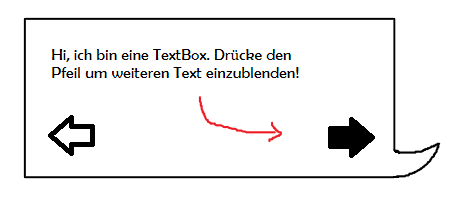
\includegraphics[scale=1.1]{bilder/Textbox.png}\\[5ex]

Nach der Einführung in die Bedienung wird nun das erste Mal eine leere Spielwelt von TLT eingeblendet. Dieser Schritt wird getan, da anhand der leeren Welt viel einfacher erklärt werden kann, welche Eigenschaften alle Welten teilen, als das eine Fülle von Text tun könnte. Generell soll unnötig viel Text immer vermieden werden, da die Motivation darunter leidet. Aussagekräftige, ergänzende Information werden trotzdem eingeblendet.

Direkt im Anschluss wird das Triangle in die Welt gesetzt, bevor es dann nach einer kurzen Erläuterung mit eigenständiger Bewegung beginnt. Auch hier soll mit zusätzlichen, kurzgehaltenen Texten erklärt werden, was dabei passiert und wieso es beispielsweise Energie kostet, Bewegung durchzuführen. Ebenfalls soll gezeigt werden, das Triangles sterben können.

Nun werden Felder eingeführt, welche verschiedene Einflüsse auf das Triangle ausüben. Die Funktion dieser soll dem Nutzer erklärt werden, in dem das Triangle demonstrativ auf die Felder bewegt wird und die Aktion direkt visuell einsehbar ist. Dabei wird dem Nutzer die Aufgabe gegeben, das Triangle zu steuern und für jeden Feldtyp zu testen, welche Konsequenz entsteht.

Nach der Erklärung der Felder wird die letzte wichtige Variable, das Sichtfeld des Triangles, erläutert. Hier ist ebenfalls eine Visualisierung eines Sichtfeldes um ein Triangle herum der beste Weg, um die Funktion und Auswirkung zu erklären. Dazu werden alle Felder, welche nicht im Sichtfeld liegen, ausgegraut. Anschließend soll der Nutzer das Triangle erneut selbst steuern können und muss mit einem Sichtfeld durch ein ihm unbekanntes Labyrinth aus Feldern zum Ziel kommen. Das verdeutlicht die Wichtigkeit des Sichtfeldes für weitere Aufgaben.

An diesem Punkt ist das Intro beendet und der Nutzer wird in das Hauptmenü versetzt. Wie genau dieses aufgebaut ist und welche wichtigen Elemente beachtet werden müssen, lässt sich in Kapitel \ref{strukturlobby} nachlesen.

\subsection{Die Lobby}

Nach dem in Abschnitt \ref{lm_intro} beschriebenen Intro gelangt der Spieler in die sogenannte Lobby. Diese ist der Mittelpunkt des Spiels und wird in folgendem Abschnitt genauer beschrieben. 

Die Lobby ist das Menü des Spiels, von dem aus der Spieler in die verschiedenen Lektionen gelangt, sowie die Referenzen einsehen und Hilfe bekommen kann. Abbildung \ref{BildLobby} zeigt den Aufbau der Lobby, welcher dem Spieler mit Hilfe der im Intro eingeführten Sprechblasen (dunkelgrün) erklärt wird. 

Dabei wird jedoch nicht einfach ein Menü integriert, über das der Benutzer seine Auswahl treffen kann. Es soll ein interaktiver Bildschirm sein, in dem die Möglichkeiten gestalterisch in die Thematik eingebunden sind. Dabei wird eine aus TLT bekannte Map aufgebaut, die der Benutzer erkunden kann. Von dort gelangt er in die verschiedenen Lektionen und gewöhnt sich sofort an die Umgebung eines Spiels. Das soll aber nicht ausschließen, dass auch ein Menü gebraucht wird, da nicht jeder Spaß an dieser Gestaltung hat. Außerdem hat es den Nachteil, dass Orientierung und mehr Zeit benötigt wird, um ein gewünschtes Ziel zu erreichen, ein Problem welches in einem Menü nicht existiert.

\begin{figure}[ht]
\centering
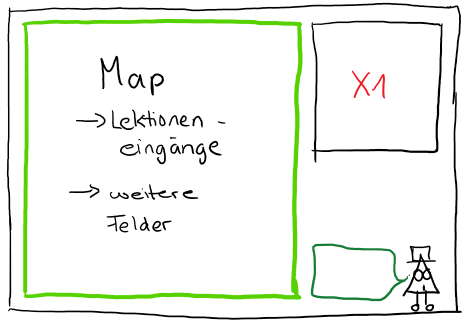
\includegraphics[scale=1.1]{bilder/Lobby.PNG}
\caption{Die Lobby}
\label{BildLobby}
\end{figure}

Der Bereich rechts oben, mit X1 betitelt, beinhaltet Platz für die Hilfe, die Referenzen und einen Shop, in dem der Spieler besondere Dinge für die im Spiel gewonnene Energie kaufen kann. Unterhalb befindet sich der Bereich, in dem eine Sprechblase immer dann abgebildet wird, wenn es etwas zu erklären gilt.

Der große Hellgrün markierte Bereich beinhaltet die Spielmap. Über diese Map gelangt der Spieler zum Beispiel in die verschiedenen Lektionen. Abbildung \ref{BildBeispielMap} zeigt, wie solch eine Map von der Art her aussehen könnte. Natürlich ist dies nur ein erster Entwurf, die reale Implementierung kann von diesem Bild abweichen. Grundlegend geht es aber darum, zu verstehen, wie die Map aufgebaut ist. Die Map ist aus folgenden Feldern aufgebaut:

\begin{center}
\label{tbl_mapFields}
\begin{tabular}{ |p{2cm} |p{3.1cm} | p{7.9cm}| c r r }
\hline
Zeichen & Feld & Bedeutung \\
\hline

\includegraphics[scale=1.1]{bilder/Wand.png} & Wände & Durch Wände kann der Spieler sein Dreieck nicht steuern. \\  
\hline

\includegraphics[scale=1.1]{bilder/Energie.png} & Energie & Energiefelder erhöhen das Energielevel des Spielers. \\
\hline

\includegraphics[scale=1.1]{bilder/Lektioneneingang.png} & Lektioneneingänge & Über die Lektioneneingänge kommt der Spieler in eine neue Lektion. \\ 
\hline
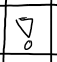
\includegraphics[scale=1.1]{bilder/Erklaerungen.png} & Erklärungen & Hier wird dem Spieler das Thema der Lektion aufbereitet erklärt. \\
\hline
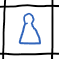
\includegraphics[scale=1.1]{bilder/Spiele.png} & Spiele & Hier finden sich die Spiele der Lektion zum nochmal spielen. \\
\hline
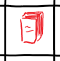
\includegraphics[scale=1.1]{bilder/referenzen.png} & Referenzen & Die passenden Referenzen zur Lektion. Durch überlaufen des Feldes wird der Bereich in der Bibliothek freigeschaltet. \\
\hline

\includegraphics[scale=1.1]{bilder/Quiz.png} & Quiz & Die Möglichkeit sein Wissen über ein Quiz zu testen.\\
\hline
\end{tabular}
\end{center}

\newpage

\begin{center}
\begin{figure}[ht]
\centering
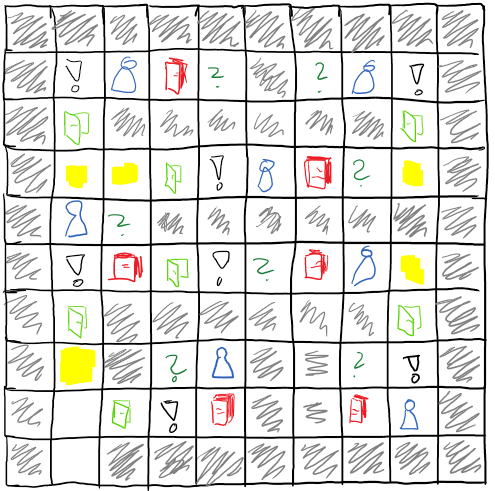
\includegraphics[scale=1.1]{bilder/BeispielMap.png}
\caption{Beispielhafte Map}
\label{BildBeispielMap}
\end{figure}
\end{center}

\newpage

Der Spieler kann mit Hilfe der Pfeiltasten seiner Tastatur das Dreieck über die Map bewegen. Befindet er sich auf einem Aktionsfeld (wie zum Beispiel einem Lektioneneingang oder dem Quiz Feld) kann der Spieler über \glqq Enter \grqq die jeweilige Aktion auslösen.

Allerdings ist zu Beginn des Spiels nicht die gesamte Map für den Spieler frei zugänglich. Je mehr Lektionen erfolgreich bestanden wurden, desto mehr ausgegraute Fläche der Map wird spielbar. Dies soll verhindern, dass der Spieler eine Lektion spielt, welche ein gewisses Vorwissen aus einem vorherigen Level benötigt. Gleichzeitig kann so auf geschickte Weise ein roter Faden durch die Lernstruktur eingebunden werden.


\subsection{Verwendete Elementen eines Educational Games}

Das Ziel des Spiels im Allgemeinen ist Wissen über AI auf eine Art und Weise zu vermitteln, welche Spaß macht. Das Ziel des Spielers ist es, am Ende in diesem Themengebiet alle nötigen Grundlagen zu beherrschen, sich mit den verschiedenen Richtungen auseinandergesetzt zu haben sowie durch nach-programmierte Codebeispiele in der Lage ist, die verschiedenen Technologien anzuwenden. 

Da es ein langer Weg bis dorthin ist und die Motivation sich etwas Neues anzueignen oftmals nicht sehr lange anhält, gibt es in dem Spiel ein Belohnungssystem, welches in leicht abgewandelter Form auf dem Energiesystem des namensgebenden Dreiecks basiert. Schließt der Spieler eine Lektion erfolgreich ab, so erhält er Energie. Ebenso wenn er zum Beispiel in einem Quiz eine Frage richtig beantwortet, oder eine Aufgabe in einer Lektion erfolgreich löst. Die gewonnene Energie kann in einem internen Shop zu Ausrüstung des Dreiecks ausgegeben werden. Das Sammeln von Energie soll dazu verhelfen, dass der Spieler Spaß hat und das Weiterspielen zum eigenen Wunsche wird, und nicht, weil der Spieler das Themengebiet lernen muss.

Ein weiteres Element aus den \textit{Educational Games} welches verwendet wird, ist das Vorgehen, dass Fehler nicht bestraft werden, sondern in gewisser Weise nötig sind, ganz nach dem Grundsatz \glqq aus Fehlern lernt man\grqq. Wenn der Spieler bei einem Quiz eine Frage falsch beantwortet, werden ihm deshalb weiterführende Informationen angezeigt. Oder wie im Kapitel \ref{lm_mlallgemein} beschrieben, muss der Spieler so lange versuchen den richtigen Weg zu finden, bis er ihn gefunden hat. Dabei lernt der Spieler aus seinen Fehlern, welche Felder er nicht betreten darf.

Um die Motivation lange hoch zu halten, einen Spannungsbogen zu ziehen und einen Ansporn zu geben, TLT bis zum letzten Level durchzuspielen, würde es sich auch anbieten, eine kleine Geschichte zu erzählen. Dies könnte zum Beispiel im Stil von den weltweit bekannten Mario-Spielen von Nintendo \cite{F_Mario_4.3.3} implementiert werden, sodass das Dreieck ein anderes Dreieck retten muss, indem es sich durch die Map spielt. Allerdings ist so eine Idee durch den zeitlich begrenzten Rahmen nicht umsetzbar. 

Auch die Möglichkeit der sozialen Interaktion in dem Spiel ist zeitlich nicht realisierbar. Dabei könnten zum Beispiel zwei Spieler gemeinsam eine Aufgabe lösen oder in einem Quiz gegeneinander antreten. Ranglisten könnten über die richtig beantworteten Fragen und erfolgreich abgeschlossene Level aufgestellt werden.

Neben diesen Elementen werden drei verschiedene Typen zum vermitteln von Lerninhalten eingesetzt. Für den Einstieg in eine neue Lektion eignen Sich Bilder und kurze Erklärungstexte am besten. Im Anschluss daran werden dann verschiedene Aufgaben geboten, durch die das Thema vertieft werden soll. Wenn ein Thema rein informativ ist und weniger Verständnisprobleme beinhaltet, eignet sich die Form eines Quiz. Hierbei können verschiedene Fragetypen eingesetzt werden, wie zum Beispiel reine Textfragen oder auswählen von passenden Bildern zu einer Frage. Als letzter Typ ist für die Lernbausteine angedacht, dass der Nutzer selbst Code schreibt, die verschiedenen Bibliotheken kennen lernt und die Ergebnisse seines Codes direkt in einer Simulation sehen kann.


\subsection{Referenzen}
\label{lm_referenzen}

Alle Informationen innerhalb von TLT beinhalten kein neu erfundenes Wissen sondern basieren auf dem vorhandenen Wissen des Themenbereiches AI. Die Quellen des in TLT enthaltenen Wissens sollen den Nutzern deshalb nicht vorenthalten werden, sodass auch für das weitere Interesse vertiefte Referenzen angeboten werden. Die Aufbereitung dieser Quellen soll dabei themenspezifisch stattfinden. Nach jeder Lektion zu einem bestimmten Thema wird deshalb das zu diesem Thema passende Zusatzmaterial verfügbar gemacht. Dabei wird keine Beschränkung auf rein wissenschaftliche Papiere stattfinden, sondern auch Codebeispiele, Tutorials und Videos sind enthalten. Aufbereitet werden sämtliche Referenzen in einem eigenen Bereich/Menü, welches einer Bibliothek ähneln soll. Dort soll nach diversen Eigenschaften wie Thema und Referenztyp gefiltert werden können. Die Bibliothek soll sich mit dem Fortschritt des Spielers in den Lektionen erweitern und soll den Nutzer dadurch animieren, in regelmäßigen Abständen nach neuen Inhalten zu sehen. Die zu einem Thema gehörigen Referenzen sind auch in unmittelbarer Nähe des Lektioneneingangs zu finden. 

Als zusätzliche Funktion ist eine eigene Einpflegung von Quellen angedacht. Da die Menge an Referenzen zu groß ist um alle zu beachten, der Nutzer aber trotzdem seine bevorzugten Informationen in der Bibliothek sammeln möchte, ist es sinnvoll dies zu ermöglichen.
\chapter{Die Lernmethodik in TLT}
\label{lernmethodik_chapter}

Dieser Abschnitt erklärt die für den Erfolg des \textit{Educational Games} notwendige Lernmethodik. Dabei wird für die verschiedenen in Kapitel \ref{lernbareTechnologien} erklärten Technologien erläutert, wie sie in TLT umgesetzt werden sollen.

\section{Artificial Intelligence im Allgemeinen}
\label{lm_aiallgemein}

Diese Lektion soll den Nutzer in das Thema AI einführen. Dabei geht es um das ganze Themengebiet und nicht nur \textit{Machine Learning}, da dieses Thema aufgrund der Wichtigkeit für dieses Projekt eine eigene Lektion bekommt.

Da es sich hier wieder um mehr oder weniger rein informative Themen handelt, wird das Format des Quiz gewählt. Zum Beispiel soll in der Lektion ein Sinn dafür entwickelt werden, wo AI überall schon zum Einsatz kommt. Dafür werden dem Nutzer mehrere Bilder wie beispielsweise das eines Schachcomputers gezeigt und er muss entscheiden, ob AI im Einsatz ist, oder nicht. Es soll klar werden, dass schon diese einfache Form einer Simulation von Intelligenz als AI bezeichnet wird. In der Lektion soll der Nutzer auch den Unterschied zwischen starker und schwacher künstlicher Intelligenz lernen können, sowie den Turing-Test und die Wichtigkeit von gut formatierten Daten für die Algorithmen kennen lernen.

\section{Machine Learning im Allgemeinen}
\label{lm_mlallgemein}

Bevor damit begonnen werden kann, Begriffe aus dem Bereich \textit{Machine Learning} zu erklären, muss zuerst erklärt werden, was \textit{Machine Learning} eigentlich ist. Ebenso muss die Frage geklärt werden, warum diese Technologie existiert und wieso es Sinn macht, sie einzusetzen. Zu guter Letzt muss aufgezeigt werden, welche Vorbedingungen für den Einsatz von \textit{Machine Learning} existieren, da es nicht ohne weiteres in jeder Umgebung verwendet werden kann.

Ein wichtiger Grundgedanke von \textit{Machine Learning} ist die Automatisierung einer oftmals für einen Menschen leicht aber langwierig zu lösenden Aufgabe. Um dem Nutzer diesen Gedanken mitzugeben, soll er das Triangle durch ein sehr leichtes Level ohne besondere Felder navigieren. Die maximale Schwierigkeit des Levels besteht darin, hin und wieder aufgrund einer Wand die gerade, direkte Strecke zu ändern und die Richtung zu wechseln. Dieses Level soll innerhalb kurzer Zeit zu lösen sein. Der Spieler wird nun gebeten, dieses Level zu lösen. Nach erfolgreichem Lösen wird ihm ein ebenso leichtes, nahezu identisches Level gegeben. Dieser Vorgang wird nun mehrmals wiederholt. Die bei dem Spieler auszulösende Reaktion soll dabei Verwirrung und Unverständnis sein. Kurz bevor er die Motivation verliert wird eine Nachricht eingeblendet, die in leicht sarkastischem Ton fragt, ob die Aufgabe Spaß mache. Die zu erwartende Antwort des Spielers ist anschließend ein geeigneter Übergang in den Themenbereich Automatisierung, da praktisch festgestellt worden ist, dass es Zeit spart, einmal einen Algorithmus zu schreiben, anstatt 100 Mal ein Level zu spielen. 

Noch fehlt in diesem Beispiel die Verbindung zu \textit{Machine Learning}, welche aber durch ein ähnliches Vorgehen geknüpft werden soll. Aufgrund der Einfachheit des oben genannte Beispiels ist es nicht nötig, mehr als einen einfachen Algorithmus zu schreiben, der die Wände meidet. Wegen dieses Umstandes ist das Beispiel nicht geeignet, um den Einsatz von \textit{Machine Learning} zu rechtfertigen. Es muss ein Beispiel gewählt werden, bei dem ein simpler Algorithmus nicht mehr mächtig genug ist. Dafür eignet sich die Klassifizierung von Bildern. Im nächsten Erklärschritt wird deshalb eine Bilderkennung simuliert, bei der der Nutzer beantworten soll, was auf einem Bild dargestellt wird. Die Zielgruppe Entwickler kennt dabei das Problem, dass nicht einfach geprüft werden kann, ob bestimmte Pixel in einem eindeutigen Muster gesetzt sind, da jedes Bild durch seine Vielzahl an Pixeln zu unterschiedlich und unregelmäßig ist, um durch simple Regeln abgebildet werden zu können. 

Die letzte wichtige Fähigkeit von \textit{Machine Learning} soll wieder mithilfe von TLT gezeigt werden. Erneut wird eine sehr simple Map gezeigt, welche aber fünf verschiedene Wege vom Start zum Ziel bietet. Jeder Weg führt aber unweigerlich an einem besonderen Bodenfeld vorbei, welches betreten werden muss. Der Spieler kennt zu diesem Zeitpunkt die in Kapitel \ref{subsubsec_oberweltregeln} vorgestellten Felder. Für dieses Beispiel werden deshalb fünf komplett neue Felder eingeführt, die nur hier gelten. Dabei ist es wichtig, dass sich an ihrem Design nicht erkennen lässt, welche Funktion sie haben. Vier von fünf Felder führen zum unweigerlichen Tod. Der Spieler hat keine andere Wahl als blind auszuprobieren, welches der Felder das Triangle nicht tötet. Dabei verwendet er seine Lernfähigkeit, der namensgebenden Aspekt, mit dem auch \textit{Machine Learning} Algorithmen ausgestattet sind. Er wird lernen, welche Felder zum Tod geführt haben und diese in Zukunft meiden. Mit einer kleinen Erklärung kann die Wichtigkeit dieser Fähigkeit für Algorithmen klargestellt werden.

Nachdem nun Eigenschaften und Nutzen erklärt wurden, muss als letztes über Vorbedingung unterrichtet werden. Nicht jede Systemumgebung lässt sich mit \textit{Machine Learning} Algorithmen zusammensetzen und nicht jedes durch Algorithmen zu lösende Problem rechtfertigt den Einsatz von AI. Als wichtigstes herauszuarbeitendes Problem kann die Datengrundlage angesehen werden, die darüber entscheidet, wie qualitativ der Algorithmus arbeitet. Es soll dem Anwender klargemacht werden, dass sauber und einheitlich aufgeschrieben Daten essentiell für einen funktionierenden \textit{Machine Learning} Algorithmus sind und deshalb immer zuerst darauf geachtet werden muss, dass diese Vorbedingung gewährleistet sind.

\section{Machine Learning Ansätze}
\label{lm_mlansaetze}
Nach dem der Spieler, wie in Abschnitt \ref{lm_mlallgemein} beschrieben, gelernt hat, was \textit{Machine Learning} ist, kann er nun die drei verschiedenen Ansätze \textit{Reinforcement Learning}, \textit{Supervised Learning} und \textit{Unsupervised Learning} lernen, welche in Abschnitt \ref{machinelearning_ansaetze} ausführlich erklärt wurden.  

Die drei Ansätze sollen dem Spieler anhand von Bildern und Beispielen jeweils kurz erklärt werden. Damit sie verinnerlicht werden, gibt es zu jedem Ansatz eine Aufgabe. Im Folgenden soll die Lernmethodik für den Ansatz \textit{Reinforcement Learning} genauer beschrieben werden. Da für die beiden anderen Ansätze  die selbe Lernmethodik gewählt wird, werden diese hier nicht mehr genauer ausgeführt.

Um die Aufgabe zu lösen muss sich der Spieler überlegen, wie der sogenannte \textit{reward} berechnet wird. Dazu bekommt er eine Ausgangssituation in Form einer Map mit den bereits bekannten Feldern. Zusätzlich erhält der Spieler eine Übersicht der Felder und je Feld die Möglichkeit einen Wert einzugeben. 

Der Spieler muss nun für jedes Feld eine Zahl festlegen. Danach kann er die Animation des Dreiecks auf der vorgegebenen Map starten. Das Dreieck läuft dann so lange, bis es keine Energie mehr besitzt. Bleibt das Dreieck stehen, bekommt der Spieler den \textit{reward}.
Der Spieler hat nun die Aufgabe, die einzelnen Zahlen der Felder so zu verändern, dass er den vorgegebenen bestmöglichen \textit{reward} erzielt. 

Somit handelt der Spieler so, wie es ein Algorithmus nach dem \textit{Reinforcement Learning} Ansatz tun würde und lernt dabei, seine Denkweise danach auszurichten.

\section{Machine Learning Techniken}
\label{lm_mltechniken}

Für verschiedene Verwendungen von \textit{Machine Learning} Algorithmen gibt es verschiedene Ansätze, die in Kapitel \ref{machinelearning_ansaetze} erklärt werden. Unterhalb dieser Ansätze können verschiedene Techniken implementiert werden, die dem Nutzer ebenso näher gebracht werden sollen. Dabei werden alle Techniken in dieser Lektion vereint und erklärt. Einen Zusammenhang zu TLT herzustellen ist dabei nicht immer möglich, da bestimme Techniken nur bei bestimmten Einsatzgebieten relevant sind.

\textit{Classification} lässt sich am besten durch eine Aufgabe erklären. Da erst eine Wissensgrundlage aufgebaut werden muss kann genau dieser Umstand dazu verwendet werden, dem Nutzer einen Einstieg zu geben. Dabei wird er mit der Fragestellung konfrontiert, warum er beispielsweise ein Objekt benennen kann, auch wenn er es noch nie gesehen hat (beispielsweise einen unbekannten Stift, der aufgrund gewisser Merkmale aber ganz klar als Stift erkennbar ist). Die Antwort liegt in seiner Wissensgrundlage, wie bestimmte Objekte aussehen. Nun kann ein Schritt weiter gedacht werden, sodass der Nutzer nun Wissensgrundlagen erstellen und bewerten darf. Dabei wird vor allem auf Kriterien wie Menge, Qualität, Gleichheit und Bezug der Datensätze bewertet. 

Ähnlich wie \textit{Classification} ist \textit{Clustering}, allerdings fehlt hier der Datensatz als Wissensgrundlage (unsupervised). Hier soll ebenfalls mittels Einbindung des Spielers ein Verständnis des Prinzips gewährleistet werden. Dazu wird dem Nutzer eine kleine Menge an Formen gegeben, die sich durch bestimmte Eigenschaften gruppieren lassen. Der Nutzer soll diese ordnen und tut damit genau das, was später ein Clustering-Algorithmus tun würde.

Regression ist ein Begriff der Mathematik, der Zahlen als Input und als Output verlangt. Hier lässt sich als gutes Beispiel die Preiskalkulation eines Produktes anhand bestimmter Eigenschaften wie Material, Größe, Produktionskosten oder Alter durch \textit{Machine Learning} anführen. Auch hier kann vom Spieler verlangt werden, in die Rolle der AI zu schlüpfen und anhand des Wissens über die Eigenschaften von Objekten ein Ergebnis zu bestimmen. 

Für alle drei Bereiche gilt die Tatsache, dass die Beispiele vereinfacht sind und in realen Situation Ausgangssituationen existieren die viel komplexer als solch eine einfache Modellierung sind. Aus genau diesem Grund übernehmen auch Algorithmen diese Aufgabe. Diese Botschaft muss dem Spieler auf jeden Fall mitgegeben werden, sonst entsteht ein falsches Bild von der Praxisanwendung der Theorie. 

\section{Neural Network}

Das Wissen, welches dem Spieler über Neuronale Netze vermittelt werden soll, kann in drei Kategorien eingeteilt werden. Den Aufbau und die einzelnen Elemente eines Neuronalen Netzes, die Funktionsweise, sowie deren Geschichte. Letztere ist nicht unbedingt notwendig und eher für interessierte Spieler gedacht. Deshalb soll es die Möglichkeit geben, dass sich der Spieler dieses Wissen in einem separat spielbaren Quiz, wie schon unter \ref{lm_einsatzgebiete} beschrieben, aneignet.

Zu Beginn der Lektion ist es zunächst wichtig, dem Spieler die einzelnen Elemente eines Neuronalen Netzes zu erklären. Dies wird, wie gewohnt, über die Sprechblasen des Dreiecks und erklärende Bilder realisiert. Dabei wird auch auf die Unterschiede von \glqq normalen\grqq{} neuronalen Netzen zu \textit{Deep Neuronal Networks} und \textit{Convolutional Neuronal Networks} eingegangen. Im Anschluss daran, hat der Spieler die Möglichkeit dieses Wissen durch ein paar Aufgaben zu vertiefen. 

Aufgabe 1: Dem Spieler werden alle Elemente eines Neuronalen Netzes zur Verfügung gestellt, welche er durch \glqq Drag and Drop\grqq{} in die richtige Reihenfolge bringen muss. Dadurch prägt sich der Aufbau eines Neuronalen Netzes besser ein.

Aufgabe 2: In dieser Aufgabe muss der Spieler ein graphisch dargestelltes (\textit{Deep/Convolutional}) Neuronales Netz zuordnen oder benennen.

Die letzte Kategorie beinhaltet die Funktionsweise von Neuronalen Netzen. Um diese möglichst einfach erklären zu können, wird nach und nach eine beispielhafte Netzwerktopologie, anhand von einem TLT-Beispiel aufgebaut. Dabei wäre es auch möglich, den Nutzer über die Auswahl von weiteren Schritten mit einzubinden. Da TLT derzeit ein \textit{Deep Neuronal Network} verwendet, wird die Funktionsweise eines Neuronalen Netzes daran erklärt.

Um das Beispiel zu vereinfachen werden statt einem Sichtfeld von neun Felder nur vier Felder genommen, und zwar: oben, unten, rechts und links. Diese gehen als Input in das Netzwerk, als Output wird eine Richtung angegeben. Eine weitere Vereinfachung besteht daraus, dass statt allen Arten von Feldern, lediglich zwei verwendet werden. 

Die Interaktion durch den Spieler könnte dabei wie folgt aussehen: Ein Teil des Netzes wird nach und nach aufgebaut. Sobald ein Muster erkennbar ist, nachdem der Aufbau erfolgt, kann der Spieler entscheiden, wie es weiter gehen müsste. Dabei erhält der Spieler sofort Rückmeldung, ob seine Entscheidung richtig oder falsch war. So hat er Teil daran, das Netzwerk aufzubauen und kann sich die daraus entstehende Funktionalität besser einprägen und ableiten.

\section{Deep Learning}

\textit{Deep Learning} ist ein Themenfeld, welches in verschiedenen Formen alle Begriffe und Technologien beinhaltet, die bisher erklärt wurden. Deshalb soll es erst nach dem erfolgreichen Abschließen aller anderen Lektionen zugänglich sein. 

Zu Beginn müssen dem Anwender allgemeine Dinge beigebracht werden, beispielsweise der Grund für die Bezeichnung \textit{Deep} und wichtige Erkennungsmerkmale eines \textit{Deep Learning} Algorithmus. Dabei soll mit dem Beispiel eines \textit{Neural Networks} gearbeitet werden. Da dem Nutzer die allgemeine Funktionsweise zu diesem Zeitpunkt schon bekannt ist, kann darauf aufbauend gezeigt werden, ab wann der Zusatz \textit{Deep} gewählt wird.

Etwas selbst machen bleibt länger im Gedächtnis, als es nur erklärt zu bekommen und sorgt außerdem auch dafür, dass der Stoff verstanden wurde. Deshalb soll in den Lektionen zu dieser Thematik eigener Code produziert werden. Dies hat den Vorteil, dass auch die anderen bisher gelernten Grundbegriffe wieder verwendet werden und das Wissen zu ihnen gefestigt wird. Für die Umsetzung dieser Methodik soll folgender Ansatz verfolgt werden:

Mithilfe einer geeigneten Bibliothek wie beispielsweise DeepLearning4Java oder Tensorflow kann gut eine im Spiel aufgesetzte Entwicklungsumgebung realisiert werden, in der der Nutzer programmieren kann. Mithilfe eines begleitenden Tutorials können die wichtigsten Ding erklärt werden. Dabei gibt es wichtige Anforderungen an das Tutorial, damit es nicht zu dem Format wird, welches das Projekt TLT verändern will. Es ist wichtig, sofort zu zeigen, was das Eingeben von bestimmtem Code auslöst. Dafür ist es nötig, eine funktionierende Simulation zu zeigen. Das Tutorial soll in der Umgebung von TLT spielen und den Nutzer vor passende Aufgaben stellen. Es soll vermieden werden, ein Anleitung abzuarbeiten, da dann die Eigenmotivation fehlt. Der Fokus soll deshalb auf Transferfragen liefern, die der Nutzer durch aufmerksames Verfolgen der Lektion beantworten kann. 

Die folgende Liste enthält eine Übersicht über mögliche Beispielaufgaben. Sie werden kurz beschrieben:

\begin{itemize}
\item Dem Nutzer wird ein \textit{Deep Neural Network} gezeigt und die Umstände seiner Implementierung erläutert. Anschließend ist es seine Aufgabe, manuell zu entscheiden, wie sich das \textit{Deep Neural Network} entwickelt. Dies kann durch eine \glqq Drag and Drop\grqq{}-Bedienung oder eigenes Schreiben von Code realisiert werden.
\item Der Nutzer soll eine bestimmte Aufgabe durch Quellcode umsetzen. \textit{"`Konfigurieren Sie das Input- und Outputlayer durch eine geeignete Wahl der Menge von Input-/Output-Neuronen"'} könnte beispielsweise eine Anweisung sein, die der Nutzer umsetzen muss. Dabei müssen ihm Informationen gegeben werden, mit denen die Aufgabe gelöst werden kann. So könnte die Größe des Triangle-Sichtfeldes ein Hinweis auf die Menge der Input-Neuronen sein und die möglichen Bewegungsrichtungen ein Hinweis auf den Output. Aufgaben in diesem Format müssen als Transferfragen umgesetzt werden. 
\item Der Nutzer bekommt ein vorhandenes \textit{Deep Neural Network} gezeigt, welches er verstehen soll. Dabei unterstützen ihn Erklärung, die aber nur als Hilfeleistung dienen und nicht die eigene Denkleistung ersetzen sollen. Diese Ausgangslage kann in mehreren Varianten durchgeführt werden. Es könnte parallel eine Simulation einer TLT-Oberwelt gezeigt werden, bei der der Nutzer entscheiden muss ob sie ein mögliches Ergebnis für das gezeigte \textit{Deep Neural Network} ist. Alternativ kann auch verlangt werden, selbst eine passende Spielsituation in TLT nachzustellen, oder eine Oberwelt zu bauen, an der sich das \textit{Deep Neural Network} verbessern kann. Dies sind alles Beispiele für einen Einsatz, welche sich auch beliebig ausbauen lassen, um noch weitere AI-Begriffe verwenden zu können.
\end{itemize}

Der Nutzer soll in dieser Themenumgebung entwickeln. Dafür ist es je nach Bibliothek nötig, eine bestimmte Programmiersprache zu wählen. Es ist erstrebenswert, dem Nutzer die Wahl zu lassen. Soll aber wie oben genannt eine eigene Simulation aufgesetzt werden, muss sich für eine Möglichkeit entschieden werden, da das Bauen verschiedener Simulationen den zeitlichen Rahmen übersteigt. Alternativ kann aber dem Nutzer mithilfe von Referenzen oder einem eigenen kleinen Kurs innerhalb von TLT die in der Simulation verwendeten Sprache näher gebracht werden, um zumindest den Einsteig zu erleichtern. Mit der Zielgruppe Entwickler muss auch nicht bei Einsteigerthemen begonnen werden, sondern es kann direkt in die Syntax eingestiegen werden. Eine Umsetzung dieser Pläne wird im Zuge dieser Arbeit aber nicht stattfinden.

\section{Einsatzgebiete}
\label{lm_einsatzgebiete}

Der Themenbereich \glqq Einsatzgebiete\grqq{} besteht hauptsächlich aus rein informativem Wissen und weniger aus Verständnisfragen. Deshalb wurde für diesen Bereich das Format eines Quiz gewählt. Der Spieler spielt sich durch das Quiz und bekommt dadurch einen guten  Überblick über die verschiedenen Einsatzgebiete von AI. Antwortet er falsch, so bekommt er weitere Informationen zu dieser Frage. Antwortet er richtig, so hat er die Option, sich weiterführende Informationen anzeigen zu lassen, oder zur nächsten Frage überzugehen. Für jede richtige Antwort bekommt der Spieler Energie.
 
Weitere Merkmale der Lektion sind:
\begin{itemize}
\item Die Lektion kann, mit der Ausnahme von AI Allgemein, unabhängig von allen anderen Lektionen gespielt werden. Es ist somit auch keine Voraussetzung für andere Lektionen.
\item Die Reihenfolge der Einheiten in der Lektion ist unwichtig.
\item Beispielprojekte oder bekannte Tools zu jedem Einsatzgebiet werden in den Referenzen bereit gestellt.
\end{itemize}
\chapter{Umsetzung}
\label{umsetzungchapter}

In diesem Kapitel soll beschrieben werden, wie die in den vorangegangenen Seiten beschriebene Planung umgesetzt wurde. Dafür wird zuerst erklärt wie eine Technologie ausgewählt wurde, bevor diese dann genauer betrachtet wird. Im Anschluss soll anhand von Beispielen konkret gezeigt werden, wie bestimmte Bausteine implementiert wurden.

Für die Umsetzung des Projektes mussten zu Beginn verschiedene Entscheidungen getroffen werden. Die unterschiedlichen Bausteine des Projektes welche essentiell sind mussten erkannt werden. Anschließend musste entschieden werden, mit welchen Technologien und Arbeitstechniken vorgegangen werden soll. Dafür wurden verschiedene Faktoren berücksichtigt:

\begin{itemize}
\item Wie aufwändig ist eine Umsetzung?
\item Lässt sich das technisch umsetzen?
\end{itemize}

Beide Faktoren und ihr Einfluss sollen kurz erklärt werden.

\paragraph{Aufwand} Der Begriff Aufwand beschreibt verschiedene wichtige Aspekte. Am stärksten wiegt für dieses Projekt der zeitliche Aufwand. Kommt die Frage auf, wie etwas umgesetzt werden soll und nach welchen Methoden gearbeitet werden muss ist es wichtig zu wissen, ob die gewählte Methodik zeitlich realisiert werden kann. Ansonsten scheitert das Projekt. Zeitaufwand wird dabei verursacht durch mangelndes Wissen über Technologie und Arbeitsweise, da dann eine Einarbeitungszeit notwendig wird. Auch ist je nach Technologie ein gewisser Planungsaufwand nötig, um beispielsweise einzelne Elemente in eine passende Form zu gießen.

\newpage

\paragraph{Realisierbarkeit} Da kein Budget investiert werden soll muss mit den Mitteln gearbeitet werden, die gegeben sind. Das gilt sowohl für Hardware als auch Software. Eine Verwendung von exklusiver und teurer Hard-/Software ist deshalb nicht vorgesehen und sollte in der Entscheidung berücksichtigt werden. Unter diesen Aspekt fällt ebenfalls, dass auch der Endnutzer eine gewisse Hardware-Limitation hat. Es kann nicht davon ausgegangen werden, dass jeder einen leistungsfähigen Computer besitzt bzw. bestimmte Software sein Eigen nennt die vielleicht benötigt wird. Deshalb muss die Verwendung von solchen Limitationen unterliegender Technologien vermieden werden.

\section{Verschiedene mögliche Ansätze}

Um die oben genannten Restriktionen einhalten zu können muss jeder Ansatz der als Umsetzungsmethodik in Frage kommt geprüft und bewertet werden. Dies soll im Folgenden näher beschrieben werden:

Der offensichtlichste Ansatz der gewählt werden kann ist der, alles selbst zu programmieren. Das bedeutet, dass jeder einzelne Bestandteil des Projekts mit möglichst viel Handarbeit erstellt wird und nicht auf ein Baukastensystem oder unzählige APIs zurückgegriffen werden soll. Auch wenn es erst so scheint, als bleibe der zeitliche Aufwand gering, da nur eine Sprache gewählt wird und mit der Entwicklung begonnen werden kann, ist das nicht korrekt. Ein genauerer, zweiter Blick zeigt diese Fehleinschätzung deutlich. Ist das Projekt weiter fortgeschritten müssen verschiedene Elemente wie eine Texteingabe oder Codeüberprüfung erstellt werden. Dies lässt sich ohne die Hilfe von APIs nur sehr schwer und zeitaufwändig realisieren. Häufig ist außerdem die eigene Programmierfreiheit durch die feste Wahl auf eine Sprache eingeschränkt, da nicht alle Funktionen ohne weiteres realisiert werden können. Als Beispiel dafür lässt sich die Codeeingabe eines Nutzers heranziehen. Soll ein gut benutzbarer Editor mit Tastenkürzeln und Syntax-Highlighting verwendet werden muss er mit einer API eingebunden werden oder selbst geschrieben sein. Letzteres ist zeitlich nicht zu bewerkstelligen, sodass nur die Alternative einer API bleibt. Schnell ist deshalb klar geworden, dass verschiedene Technologien ein großes Projekt ergeben werden. Allerdings entstehen auch bei diesem Ansatz Nachteile. Nicht jede API oder Technologie ist kompatibel miteinander. Jede hat ihren eigenen Verwendungszweck, so das eine Auswahl getroffen werden muss. Für einen langwierigen Entscheidungsprozess ist jedoch nicht genug Zeit, sodass ein grober Blick ausreichen muss, auch wenn ein Fehlgriff schlechter vermeidbar ist. Der zweite Nachteil, der ebenfalls Grund für eine schnelle Auswahl ist, stellt die Benutzung dar. Nicht immer ist das Wissen darüber vorhanden, sodass erst der Umgang gelernt werden muss. Auch hier muss mit einem großen Zeitaufwand gerechnet werden, der zur Folge hat das nicht sofort mit Ergebnissen gerechnet werden kann. Deshalb sollten zu viele verschiedene Methoden und Technologien genauso vermieden werden wie die Einschränkung auf nur eine einzige. Eine Mischlösung aus beiden Varianten, also einer eigenen Entwicklung mit möglichst wenig Fremdeinwirkung und verschiedene Technologien für verschiedene Bereiche muss gefunden werden.

\section{Unity}

Unity ist ein Framework für Spiele-Entwickler, welches sich durch seine Bekanntheit und Größe auszeichnet. Durch die gezielte Ausrichtung auf das Erstellen von Spielen bietet es sich an, es zur Erstellung eines Educational Games zu verwenden. Viele interne oder durch Plugins nachträglich erzielbare Funktionen können mittels "What You See is What You Get"-Prinzip dazu verwendet werden, fast alle Aufgaben zu erfüllen die benötigt werden. Bereits mit Unity erstelle Projekte zeigen gut, wie komplex es dabei werden kann. Mittels CSharp-Skripten kann eigener Code dazu verwendet werden, nicht ganz so offensichtliche Funktionen zu realisieren. Unity ist dabei am besten mit "leicht zu lernen, schwer zu meistern" zu beschreiben. Simple Spiele sind schnell erstellt, komplexe Aufgaben brauchen jedoch einen erheblich höheren Zeitaufwand. Dadurch wird es einfacher, einen funktionierenden Prototypen zu erstellen. Ob der Aufwand niedriger ist als eine Entwicklung mit einer anderen Herangehensweise kann im Bezug auf eine komplexe Aufgabe nicht aufgezeigt werden. Im Fokus dieser Arbeit steht die Erstellung eines Prototypes, der aufzeigt wie das finale Endprodukt aussehen soll. Dies sollte sich mit Unity realisieren lassen. Dazu wird zuerst die Funktionsweise von Unity betrachtet.

\newpage

\section{Funktionsweise von Unity}

In diesem Abschnitt sollen die kennengelernten Mittel zum Umgang mit Unity beschrieben und erklärt werden. Dabei besteht nicht der Anspruch Unity vollständig zu erklären. Das Ziel hingegen ist, zu zeigen, wie der Grundlegende Aufbau von Unity ist und mit welchen Komponenten und Funktionen im laufe der Erstellung des Prototyps gearbeitet wurde.

\subsection{Die Unity UI}

Unity hat wie jede Entwicklungsumgebung mehrere Fenster mit verschiedenen Funktionen. Die wichtigsten (und am häufigsten genutzten) Fenster sollen im folgenden kurz beschrieben werden:

\begin{itemize}
\item \textit{Project}: Über das Fenster \textit{Project} wird zu den Assets sowie zu anlegbaren Favoriten navigiert. Um den Überblick über die Assets nicht zu verlieren lohnt es sich, sie in einer Ordnerstruktur zu organisieren. Wir haben die Ordner Prefabs, Scenes, Scripts, Sounds, Sprites und Textures angelegt. Deren Inhalt wird im laufe des Abschnittes noch erläutert werden.
\item \textit{Hierarchy}: In diesem Fenster werden alle Elemente/Objekte einer geladenen Szene hierarchisch nach ihren Abhängigkeiten mit Namen angezeigt. Bei einem Klick auf ein Objekt, wird dieses in dem Fenster \textit{Scene} markiert.
\item \textit{Scene} und \textit{Game}: Im Fenster \textit{Scene} kann der aktuelle Stand des Spiels, beziehungsweise der geladenen Szene, eingesehen werden. Das bedeutet, dass alle Objekte der Szene anklickbar sind und daraufhin im \textit{Inspector} Fenster untersucht werden können. Per Drag and Drop können der Szene weitere Elemente aus der \textit{Project} Übersicht hinzugefügt werden.
Wenn auf den Play Button (oben in der Mitte der UI von Unity) gedrückt wird, wechselt Unity automatisch in das \textit{Game} Fenster und die aktuelle Szene kann als \glqq echtes \grqq Spiel getestet werden.  \newpage
\item \textit{Inspector}: Wird ein Objekt in dem Fenster \textit{Scene} oder aus der \textit{Hierarchy} ausgewählt, können weitere Informationen zu dem Objekt in diesem Fenster eingesehen und verändert werden. Zum Beispiel Größe, Position, Farbe und Verhalten. Letzteres kann durch Verknüpfen eines Scripts mit diesem Objekt realisiert werden. 
\item \textit{Console}: In diesem Fenster werden alle Texte und Fehlermeldungen ausgegeben.
\end{itemize}

\subsection{Was für Elemente verwendet werden können}
\label{Elemente}

Um das Spiel mit Unity zu gestalten, gibt es verschiedene Elemente, die verwendet werden können. 

\subsubsection{Szene}

Den grundlegenden Baustein stellt dabei die Szene dar. Diese enthalten die verschiedenen Umgebungen und Menüs des Spiels, wobei jede Szene als eigenes Level gesehen werden kann. Auf einer Szene können verschiedenen \textit{GameObjects} angeordnet werden. Per C\# Skript (siehe Beispiel in Abschnitt \ref{u_beispiele}) kann zwischen den verschiedenen Szenen gewechselt werden. Doch was sind eigentlich die mehrfach genannten Game Objekte? ~\cite{F_6.3.2.1_Scenes}

\subsubsection{Game Objekt}
Das Game Objekt ist das wichtigste Konzept in der Gestaltung von Szenen. Jedem Objekt des Spiels liegt ein Game Objekt zu Grunde. Allerdings kann ein leeres Game Objekt nichts alleine tun. Um ihm eine besondere Bedeutung oder Verhalten zu geben, muss dem Game Objekt eine oder mehrere Komponenten (je nach Objekttyp welcher erstellt werden soll) hinzugefügt werden. Ein Game Objekt kann zum Beisiel in der Hierarchie per Rechtsklick erstellt werden. Hier gibt es die Möglichkeit ein leeres Game Objekt zu erstellen, oder schon vorgefertigte Objekte zu verwenden. Ist es erstellt können dem Objekt Komponenten hinzugefügt werden, damit es zu dem werden kann, zu dem es bestimmt ist. Die Komponente \textit{Transform} muss in jedem Game Objekt enthalten sein. Deswegen wird sie automatisch zu einem neu erstellten Objekt hinzugefügt und kann auch nicht gelöscht werden. Die Komponente legt Position und Ausrichtung fest. ~\cite{F_6.3.2.2_GameObjekts}

\subsubsection{Komponenten}
Komponenten sind zum Beispiel Effekte, Licht, Text, Formen, Ton, Video oder Skripte. Mit Hilfe der Skripting API können auch eigene Komponenten erstellt werden. Komponenten stellen, wie oben schon angedeutet, die eigentliche Funktionalität von Game Objekten. Zum Beispiel enthält jede erzeugte Szene von Beginn an das Main Camera Game Objekt. Dieses \glqq normale\grqq Game Objekt wird durch die hinzugefügte Komponente \textit{Camera Component} erst zur Kamera, durch die der Spieler die Spielwelt sehen kann.

Es gibt mehrere Möglichkeiten um eine Komponente zu einem Game Objekt hinzuzufügen. Zum einen über das Component Menü in der Werkzeugleiste, oder insofern das Objekt gerade ausgewählt ist, über den Inspektor und die Schaltfläche \textit{Add Component}. 

Eine Komponente mehrere Properties besitzen. Diese sind entweder vom Typ \textit{value} oder \textit{reference}. Values sind einfache Werte, welche direkt im Inspektor angepasst aber auch im laufenden Spiel über eigene Skripte verändert werden können. References stellen Verweise auf jegliche Art von Game Objekten dar. Diese können einfach per Drag and Drop hinzugefügt werden.

Unity bietet eine sehr gute Dokumentation über die verschiedenen Komponenten. Die jeweilige \textit{Component Reference Page} ist auch über das Fragezeichen-Symbol im Inspector neben dem Komponentennamen erreichbar. \cite{F_6.3.2.3_Komponenten}

\subsubsection{Assets und Prefabs}
Ein Asset ist eine Repräsentation von irgendeinem Item, welches im Unity Projekt verwendet werden kann, sozusagen der Überbegriff.

Prefabs sind ein Asset Typ, der es dem Entwickler erlaubt, Game Objekte komplett mit allen Komponenten und Skripten als eine \glqq Vorlage \grqq zu speichern. Das ist besonders dann hilfreich, wenn das Game Objekt sehr oft verwendet werden soll. Denn ein Prefab hat den Vorteil (vor normalem Copy/Paste), dass wenn das Prefab verändert werden sollte, alle Instanzen die davon in der Spiele Welt existieren entsprechend mit verändert werden. ~\cite{F_6.3.2.4_Prefabs} 

\subsubsection{Sprites}

Sprites sind einfache graphische 2D Objekte, also Bilder, welche einem Game Objekt zugeordnet werden können. ~\cite{F_6.3.2.5_Sprites}

\subsubsection{Skripte}
Möchte der Entwickler einem Game Objekt Funktionalität geben, welche sich noch nicht in vordefinierten Komponenten findet, hat er die Möglichkeit diese in Form von einem Skript selbst zu definieren. Unity unterstützt zwei verschiedene Sprachen: C\# und UnityScript. Durch Skripte können beispielsweise Game Events getriggert werden, Komponenten Properties während der Laufzeit des Spiels verändern und auf Nutzereingaben reagieren. ~\cite{F_6.3.2.6_Skripte}

Ein Script kann wie jede andere Komponente ebenfalls über den \textit{Add Component} Button im Inspektor hinzugefügt werden. Sollte es sich bei dem Game Objekt um ein anklickbares Objekt handeln, kann im Inspektor ebenfalls definiert werden, welches Skript und welche Methode aus dem Skript als Folge eines Klicks ausgeführt werden sollen.

In Abschnitt \ref{u_beispiele} wird auf den Aufbau und die Funktion der Skripte noch näher eingegangen.


\subsection{Zusammenarbeit}
Da dieses Projekt zu zweit entwickelt wird, stellte sich natürlich auch die Frage, wie der Code geteilt und versioniert werden kann. Eine Verwendung von GitHub, einer Plattform die genau diese Aufgabe erfüllt, wurde kurz nachgedacht. Da dazu aber die Verwendung von Add-ons und diverse Einstellungen nötig waren wurde aufgrund der einfachen Handhabung und des geringen Konfigurationsaufwandes eine zweckmäßige Alternative gesucht. Diese fand sich in Unity selbst, denn genau für die Frage der Teamzusammenarbeit bietet Unity von Haus aus die Funktion Collaborate an. Auf der Homepage wird die Funktion wie folgt beschrieben: \glqq Collaborate ist ein einfacher Weg für Teams, ihr Unity-Projekt zu speichern, zu teilen und zu synchronisieren. Collaborate ist Cloud-gehostet und benutzerfreundlich, sodass das gesamte Team zum Projekt beitragen kann, unabhängig von Standort und Rolle. \grqq ~\cite{F_6.3_UnityCollab} 

\section{Beispielhafte Implementierung einer Funktion in Unity}
\label{u_beispiele}
In diesem Abschnitt werden einige Beispiele aus dem Projekt in Form von Code und Erklärungen gezeigt, um einen Überblick über die Implementierung zu geben, sowie die Handhabung von Unity und der Scripting API aufzuzeigen.

\subsection{Beispielhalfter Aufbau eines Skripts}
Listing \ref{lst:BeispielSkript} zeigt ein in Unity neu erstelltes Skript mit dem Namen \textit{BeispielSkript}. Gut zu erkennen ist, dass der Klassennamen immer dem Skriptnamen entsprechen muss, damit das Skript als Komponente an ein Game Objekt gebunden werden kann. Jedes Skript muss die Klasse \textit{Monobehaviour} implementieren, wenn eine Verbindung zu den inneren Funktionen von Unity aufgebaut werden soll.

Per Default hat ein Skript zwei Funktionen. Diese können, müssen aber nicht verwendet werden. Die Funktion \textit{Start()} wird aufgerufen, bevor das Spiel beginnt. Da in Unity Objekte nicht durch einen selbstdefinierten Konstruktor erstellt werden, sondern von Unity selbst, ist stattdessen hier der Platz um nötige Initialisierungen durchzuführen. In der Funktion \textit{Update()} können Aktionen abgehandelt werden, die während dem Spielen auftreten, wie zum Beispiel Benutzereingaben oder eine Bewegung des Spielers.

\lstset{style=sharpc}
\begin{lstlisting}[caption=Beispiel Skript, label=lst:BeispielSkript]

using System.Collections;
using System.Collections.Generic;
using UnityEngine;

public class BeispielSkript : MonoBehaviour {

	// Use this for initialization
	void Start () {		
	}	
	// Update is called once per frame
	void Update () {	
	}
}
\end{lstlisting}

\subsection{Szenenwechsel}
Wie in Abschnitt \ref{Elemente} beschrieben, sind Szenen wichtige grundlegende Bausteine für die Erstellung eines Spiels. Da ein Spiel nicht nur aus einer Szene besteht, sondern aus einer Vielzahl dieser, sollte es die Möglichkeit geben, zwischen den verschiedenen Szenen wechseln zu können. Hierfür bietet die Unity Scripting API eine einfache Funktion:

\lstset{style=sharpc}
\begin{lstlisting}[caption=Szenenwechsel, label=lst:Szenenwechsel]

public class LoadSceneOnClick : MonoBehaviour {
	
    public void LoadByIndex(int sceneIndex) {
        SceneManager.LoadScene(sceneIndex);
    }
}

\end{lstlisting}

In Listing \ref{lst:Szenenwechsel} ist die selbstgeschriebene Funktion \textit{LoadByIndex} für den Szenenwechsel zu sehen. Hierfür wurde die Methode \textit{LoadScene(sceneIndex)} des SceneManagers verwendet. Ruft ein Game Objekt oder ein anderes Skript die eigene Methode des Skripts \textit{LoadSceneOnClick} auf, wird zu der Szene mit dem angegebenen Index gewechselt. 

Welche Szene welchen Index besitzt, kann in den Build Settings festgelegt werden (Abbildung \ref{BuildSettingsPic}). Hier müssen alle Szenen, welche verwendet werden sollen, eingetragen werden. Jede neue Szene erhält dabei einen eindeutigen Index. Durch anklicken und ziehen einer Szene kann die Reihenfolge und damit auch der Index verändert werden. Der beim Hinzufügen einer Szene angelegte Index ist also nicht endgültig.

\begin{figure}
\centering
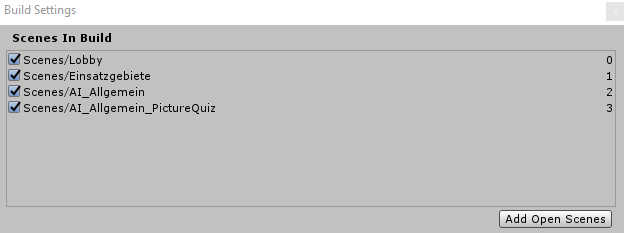
\includegraphics[scale=0.85]{bilder/BuildSettings.PNG}
\caption{Build Settings}
\label{BuildSettingsPic}
\end{figure}

\subsection{Die Lobby}

\subsection{Ein Quiz}
In diesem Abschnitt wird etwas ausführlicher beschrieben, wie ein Quiz implementiert werden kann. Er stellt nicht den Anspruch, die einzig richtige Art und Weise zu sein, wie das möglich ist. Damit am Ende nicht nur eine unbewegliche Oberfläche heraus kommt, braucht es zusätzlich zu dieser noch ein paar Skripte und das EventSystem (vorgefertigtes Game Objekt), welches für die Verarbeitung von Events in der Unity Szene zuständig ist. Sonst existiert in der Quizszene nur noch die \textit{Default Kamera}, welche aber unverändert bestehen bleiben kann.

\subsubsection{Die Oberfläche}
Alle Elemente der Oberfläche werden auf dem sogenannten Canvas angeordnet. Dieser dient wie in Java Swing ein Frame als Container für alle weiteren Game Objekte. In Abbildung \ref{QuizOberflaechePc} ist die Quizoberfläche im Szenenfenster zu sehen. Das Canvas ist durch die vier blauen Punkte an den Ecken gekennzeichnet. (Hinweis: So sieht es im Szenenfenster immer aus, wenn ein Element in der Hierarchie oder direkt in der Szene selektiert wurde). Die sechs hellen Rechtecke sind Button, denen jeweils ein Text zugeordnet wurde. Die beiden dunklen Bereiche sind Panel, denen ebenfalls ein Text zugeordnet wurde. 

Wie die gesamte Szene aufgebaut ist, kann im Fenster Hierarchie gesehen werden (Abbildung \ref{HierarchiePc}). Eine weitere Komponente, welche bisher verschwiegen wurde, ist der GameManager. Dieser ist ganz oben in der Hierarchie zu sehen und stellt einfach ein leeres Game Objekt dar, welches mit dem in Abschnitt \ref{QuizSkripte} erklärten GameManager-Skript verknüpft wird. Sobald alle Funktionen implementiert sind, können über dieses Game Objekt die verschiedenen Fragen und die dazugehörigen Antworten im Inspektor eingegeben werden. Auch die Verknüpfung zwischen den im Skript definierten Variablen und den UI Komponenten findet in diesem Game Objekt statt.

\begin{figure}
\centering
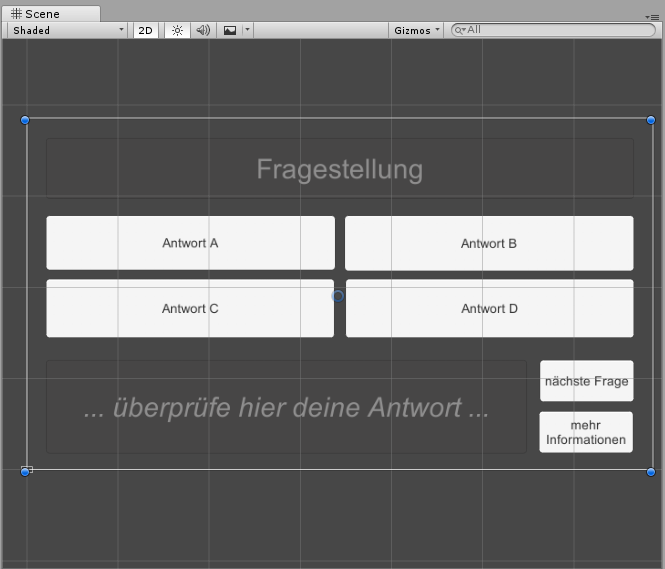
\includegraphics[scale=0.8]{bilder/QuizOberflaecheSzene.PNG}
\caption{Die Quiz Oberfläche im Szenen Fenster}
\label{QuizOberflaechePc}
\end{figure}

\begin{figure}
\centering
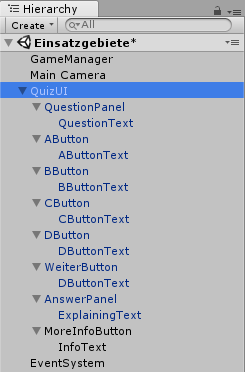
\includegraphics[scale=1]{bilder/Hierarchie.PNG}
\caption{Hierarchie}
\label{HierarchiePc}
\end{figure}

\subsubsection{Die Skripte}
\label{QuizSkripte}
Damit die Buttons und die Panel auch mit Funktionen belegt sind, müssen diese mit Skripten verbunden werden, sonst bleibt unsere UI unbeweglich und somit nicht spielbar.

Zwei Skripte sind essentiell. Das Skript \textit{Question} ist lediglich ein Model, über welches später aus dem \textit{GameManager-Skript} auf die verschieden Fragen und Antwortet zugegriffen werden soll. Deshalb weicht der Aufbau des C\# Skriptes auch leicht von der vorgestellten Art und Weise ab. 

Etwas komplexer ist das Skript für den GameManager. Neben sieben verschiedene Funktionen um dem Quiz seine \glqq Seele\grqq zu geben gibt es einigen Variablen- und Komponentendeklarationen. Variablen halten zum Beispiel die aktuelle Frage oder ein Array aller Fragen. Mit Komponentendeklarationen sind variablen gemeint, die auf eine Komponente innerhalb der UI verweisen. Zum Beispiel kann der Button für weitere Informationen oder der Text des Antwortpanels mit dem Code aus Listing \ref{lst:ButtonMoreInformation} angesprochen und kontrolliert werden.

\lstset{style=sharpc}
\begin{lstlisting}[caption=Deklaration von UI Komponenten, label=lst:ButtonMoreInformation]
[SerializeField]
private Button moreInfoButton;

[SerializeField]
private Text answerText;
\end{lstlisting}

Das allgemeine Prinzip ist, dass zunächst alle vorhandenen Fragen aus dem GameManager in ein Array geladen werden. Um das doppelte stellen von Fragen zu vermeiden wird eine Liste von ungefragten Fragen angelegt, welche beim Start gefüllt wird. Wurde eine Frage richtig beantwortet, kann diese aus der Liste gelöscht werden.

Folgende Aufzählung gibt einen kurzen Überblick, welche Funktionen das Skript enthält:

\begin{itemize}
\item Start(): Füllen der Variablen mit den Frage/Antworten aus dem GameManager Objekt und Vorbereiten der UI Komponenten
\item SetCurrentQuestion(): Eine Frage aus den unbeantworteten Fragen auswählen, als aktuelle Frage festlegen und auf der UI anzeigen. Wird von Start() aufgerufen. Ruft seinerseits SetButtonText() auf.
\item SetButtontext(): Belegt die Button mit den jeweiligen Antwortmöglichkeiten.
\item TransitionToNextQuestion(): Wird aufgerufen wenn der Button \glqq nächste Frage \grqq geklickt wird. Wenn noch Fragen vorhanden sind, wird die nächste Frage geladen, wenn nicht, dann wird zur nächsten Szene gewechselt.
\item ShowMoreInformation(): Wird aufgerufen wenn der Button \glqq mehr Informationen \grqq geklickt wird. Zeigt den in der Frage hinterlegten Text mit weiteren Informationen auf der Oberfläche an.
\item DisableMoreInformationButtonIfNull(): Sollten keine weiteren Informationen vorhanden sein, wird der Button disabled. Wird von der Funktion UserSelectQuestion() aufgerufen.
\item UserSelectQuestion(): Diese Funktion prüft, ob der Nutzer die richtige Antwort ausgewählt hat.
\end{itemize}

Um das Zusammenspiel von UI Komponenten und Skript zu verdeutlichen, wird im Folgenden die Funktion ShowMoreInformation() (Listing \ref{lst:ShowMoreInformation}) genauer betrachtet.

\lstset{style=sharpc}
\begin{lstlisting}[caption=Verwendung von UI Komponenten im Skript, label=lst:ShowMoreInformation]
public void ShowMoreInformation()
{
    string moreInformationText = currentQuestion.moreInformation;
    answerText.color = Color.cyan;
    answerText.fontSize = 14;      
    answerText.text = moreInformationText;
}
\end{lstlisting}

Zunächst wird der Informationstext aus der aktuellen Frage ausgelesen und in die Variable \textit{moreInformationText} geschrieben. Die zwei Zeilen darauf sind für Farbe und Schriftgröße zuständig. In der letzten Zeile wird nun noch der Inhalt dem Textfeld zugewiesen.

Wie oben schon beschrieben, wird die Funktion durch den Klick des Buttons ausgelöst. Dies wird dadurch erreicht, dass dem Button im Inspektor diese Funktion hinzugefügt wird. Da das Game Objekt ein Button ist, enthält er im Inspektor das Feld onClick(). Hier kann wie in Abbildung \ref{onClickPc} zu sehen, zunächst ein Skript hinzugefügt und anschließend daran eine Funktion aus dem Skript ausgewählt werden (in diesem Fall die Funktion ShowMoreInformation()).

\begin{figure}
\centering
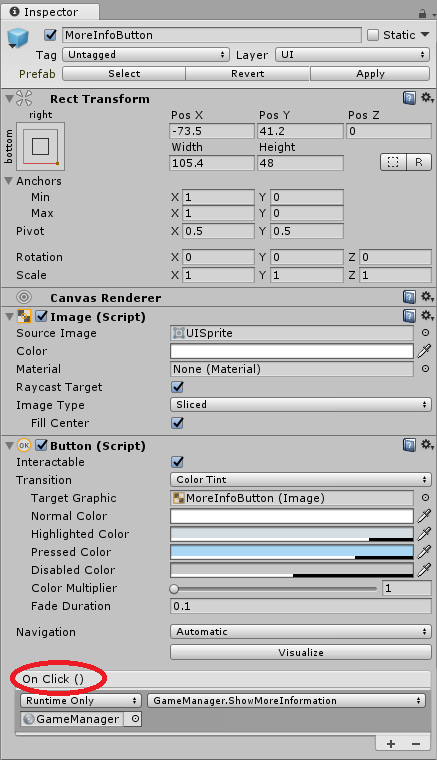
\includegraphics[scale=0.9]{bilder/OnClick2.PNG}
\caption{onClick() Methode im Button}
\label{onClickPc}
\end{figure}

\chapter{Fazit}
\label{fazitChapter}
In diesem Kapitel soll in Form eines Rückblickes betrachtet werden, inwiefern die Arbeit als gelungen betrachtet werden kann. Dazu wird zuerst Vorgehen, Teamentwicklung und Ergebnis evaluiert, bevor mit einem Ausblick auf zukünftige Möglichkeiten abgeschlossen wird.

\section{Evaluation der Studienarbeit}

Die Studienarbeit ist an diesem Punkt zeitlich abgeschlossen und deshalb soll ehrlich und kritisch bewertet werden, was als gut und was als schlecht anzusehen ist. Dafür wurden verschiedene Aspekte betrachtet:

\paragraph{zur Entwicklung:} Das Ergebnis in Form des Prototypes ist akzeptabel, hätte aber unter besseren Umständen einer finalen Form deutlich näher kommen können. Gründe für diesen Umstand gibt es verschiedene, als wichtigster muss zuallererst festgehalten werden, dass der Aufwand von Unity unterschätzt wurde. Tatsächlich ist es nicht schwierig, simple Programme zu erstellen. Diese sind aber weit von einem fertigen Produkt entfernt und wirken weder aufbereitet noch poliert. Mehr als ein kleines Spiel lässt sich ohne große Aufwand nicht realisieren. Des Weiteren ist sehr viel Zeit in Planung und Experimente geflossen. Als festgelegt wurde, dass Unity das Mittel der Wahl wird, ist bereits in verschiedenen Technologien mehr oder weniger viel entstanden, welches aber an Wichtigkeit verlor. Dem höheren Zweck einer wissenschaftlichen Arbeit, dem Sammeln von Erfahrung und dem Erforschen von Möglichkeiten hat dies jedoch nicht geschadet. Einzig die in der Arbeit entstandene Anwendung leidet unter der nicht optimalen Ausnutzung der gegebenen Zeit. Deshalb lässt sich zusammenfassend sagen, dass falls in Zukunft weiter daran gearbeitet werden sollte, dann müsste noch viel getan werden, um zu einem fertigen Produkt zu gelangen. 

\paragraph{zur Teamarbeit:} Die Studienarbeit wurde von zwei Personen erstellt. Das bringt mit sich, dass über die weiteren Schritte kommuniziert werden muss und dass Entscheidungen getroffen werden. Als Einzelperson lässt sich dieser Vorgang ohne Aufwand umsetzen, in einer Gruppe wird das jedoch in manchen Situationen zu einer Herausforderung. Je nach Team muss über Entscheidungen lange diskutiert werden. Die Arbeit in einer Gruppe von zwei Personen war in diesem Fall jedoch ein angenehmer Vorgang. Bis auf grundlegende Festlegungen zu Technologie und Methodik war das Vorgehen meistens klar und bedarf keiner langen Diskussion. Der Vorteil von mehr Arbeitskraft konnte deshalb zufriedenstellend ausgenutzt werden. Mehr Personen die mitarbeiten hätten einen höheren Kommunikationsaufwand bedeutet, weniger Personen hätten ein schlechteres Ergebnis zur Folge gehabt. Abschließend lässt sich also feststellen dass die Aufgabe gut für eine Teamarbeit geeignet war.

\paragraph{zur agilen Vorgehensweise:} Zum Beginn der Arbeit erschien der Aufwand, der durch das agile Vorgehen verursacht wurde unverhältnismäßig groß. Ein Backlog musste erarbeitet werden, ein Tool zur ordentlichen Verwaltung musste ausgewählt werden und sämtliche Stories und Tasks mussten eingetragen werden. Dies verlief nicht immer so automatisiert wie es von verschiedenen Aussagen versprochen wird. Nach einigen Wochen hatte sich jedoch schnell eine gewisse Routine in der Arbeit mit der agilen Methode eingespielt, sodass der zusätzliche Aufwand akzeptabel klein wurde. Zusätzliche Gründe für den doch eher ungewöhnlichen Aufwand zu Beginn waren unter anderem eine gewisse Unerfahrenheit, was häufig Zeit kostete. Außerdem musste eine Person des Teams für eine Wahlpflichtveranstaltung zusätzlich Dokumente anfertigen, um in dem Fach die Prüfung zu bestehen, wurde auch dadurch Zeit beansprucht. Nachdem diese Prüfungsleistung erbracht war und die gewissen Startschwierigkeiten beseitigt waren, half die agile Methode aber geordneter und vor allem auch disziplinierter an der Thematik zuarbeiten. Es hat geholfen, verschiedene Aufgaben aufzuteilen zu können, da dadurch weniger unerwartetes passierte. Zusammenfassend ist es sinnvoll, darüber nachzudenken der agilen Methode eine Chance zu geben, wäre auf dieses Projekt bezogen aber absehbar gewesen dass der Aufwand zu Beginn so groß ist, wäre die Entscheidung sehr wahrscheinlich anders ausgefallen.

\paragraph{zum in Kapitel \ref{timetrackingParagraph} erstellten Timetracking:} Als Gesamtaufwand für die Arbeit kann eine Zeitmenge von 165 Stunden festgehalten werden. Dabei gibt es Unterschiede zwischen den am Projekt beteiligten Personen von 20 Stunden. Gründe dafür sind zum einen unterschiedliche Wissensgrundlagen und unterschiedliche Arbeitsmethodiken während der Entwicklung. Die in vier Bereiche kategorisierten Zeiten zeigen, dass bis auf größere Unterschiede in der Entwicklung keine nennenswerten Differenzen existieren. Allgemeine Aussagen lassen sich im Anschluss jedoch trotzdem nicht treffen, da sehr situationsbezogen geurteilt werden muss. Mehr Entwicklungszeit könnte schlechteres Vorwissen, aber auch gründlichere Arbeit als Ursache haben. Außerdem ist nur mittelmäßig erkennbar, ob wirklich alle Tasks passend kategorisiert wurden und Zeiten korrekt eingeflossen sind. Deshalb soll an dieser Stelle kein Urteil gefällt werden. Stattdessen soll in kurzer Ausführung analysiert werden, wie während der Arbeit vorgegangen wurde. Dabei zeigt sich, dass in Summe die meiste Zeit für das Schreiben der Arbeit aufgebracht wurde, was keine Überraschung ist. Der Aufwand, 70 Seiten zu produzieren überwiegt in diesem Fall den, der für das Erstellen eines Prototypes notwendig war. Nicht zu verachten ist jedoch auch der Aufwand der für die Vorarbeit aufgewendet werden musste. Wünschenswerterweise  hätte weniger Zeit dafür reichen müssen, macht das Schaffen der Grundlage in dieser Arbeit doch einen Gesamtaufwand von fast einem Viertel aus. Ebenfalls lässt sich zeigen, dass sehr wenig getestet wurde, was unter anderem auf die Wahl der Technologie und die Ressourcenverteilung zurückgeführt werden kann. In einem echten Projekt hätte dafür auf jeden Fall mehr Zeit investiert werden müssen. Im Großen und Ganzen belegt das Aufschlüsseln der Zeiten die im Fazit bisher genannten Punkte sehr gut. Im Anhang findet sich außerdem noch ein weiteres Diagramm (Abb. \ref{RTimeReport}), welches ebenfalls dort erläutert wird.

\paragraph{zum in Kapitel \ref{riskmanagementchapter} erstellten Risikomanagement:} Das Risikomanagement welches zu Beginn der Arbeit ausgearbeitet wurde hat immer vor Augen geführt, inwiefern es um die möglichen Risiken steht. Grundvoraussetzung dafür war allerdings, dass es auch immer betrachtet und angepasst wurde. Dies wurde während der Studienarbeit nur unregelmäßig getan. Trotzdem sind keine bedrohlichen Risiken aufgetreten, wobei das Wissensproblem deutlich zu spüren war. Es hat viel Zeit gekostet, sich einzulesen. Die Klausuren wurden weitestgehend über das ganze Semester verteilt, sodass eigentlich immer etwas zu tun war. Das war angenehm im Bezug auf Klausuren, allerdings wurde dadurch in Summe weniger in die Studienarbeit investiert. Hardwareprobleme traten keine auf und auch krankheitsbedingt gab es keine Ausfälle. Die Kommunikation war nicht immer einfach, da verschiedene Ansichten hin und wieder zu einer Kollision der Teamkollegen führte. Es gab aber auf die ganze Arbeit gesehen keine großen Schwierigkeiten aufgrund dessen. Das Risiko mit dem größten Einfluss war mit Sicherheit die Zielsetzung, welche zu groß dimensioniert war. Nur mit einem erheblichen Mehraufwand über die angedachte Menge an Arbeit hinaus wäre es gelungen, ein finales Produkt zu entwickeln. 

Die Methode Risikomanagement an sich erfüllte ihren Zweck und sollte auch in zukünftigen Projekten verwendet werden. Mit einer regelmäßigeren Bearbeitung der Risiken würde das Vorgehen zusätzlich an Nutzen gewinnen. Im Anhang findet sich eine Tabelle die für jedes Risiko noch einmal genauer zeigt, ob es eingetreten ist und wie damit umgegangen wurde.

\paragraph{zu sonstigen nennenswerten Dingen:}
Zu Beginn wirkte der zeitliche Rahmen von sechs Monaten sehr lang, da bisherige Arbeiten mit ähnlichem Umfang nur drei Monate zugesprochen bekamen. Natürlich muss beachtet werden dass im Gegensatz zu den anderen Arbeiten nicht täglich acht Stunden dafür verwendet werden können. Aufgrund von Vorlesungen und Klausuren stellte sich am Ende heraus dass eigentlich deutlich weniger Zeit zur Verfügung stand. Im Großen und Ganzen kann das Ergebnis für die vorhandene Zeit als zufriedenstellend bewertet werden. Bereits im Bereich Entwicklung wurde über die Bewertung des Ergebnisses gesprochen.
Ebenfalls schwierig stellte sich das Anlesen und Herausschreiben der Thematik AI heraus. Viele verschiedene Auslegungen machten es nicht einfach, eine klare Meinung zu vertreten, die unter gutem Gewissen in einem Lernspiel eingebaut werden konnte. Oft musste viel Zeit für die Suche und Anpassung einer gefundenen Quelle aufgebracht werden, nachdem auch darüber diskutiert wurde. Das hätte mit einem klarer definierten Thema weniger Schwierigkeiten zur Folge gehabt
Ein wenig schade ist die Tatsache, dass viele Tätigkeiten wie beispielsweise das Anlesen von Wissen oder Ausprobieren von verschiedenen Dingen nicht aus der sichtbaren Lösung erkenntlich werden. Das lässt die Euphorie über den Abschluss der Arbeit etwas nüchterner ausfallen.

\section{Ausblick}

Als Abschluss der Arbeit soll darüber nachgedacht werden, wie dieses Projekt weitergehen würde, wenn eine Weiterarbeit zustande kommt. Dabei gibt es drei Themen die angegangen werden sollten:

\begin{itemize}
\item Der Prototyp
\item Die Lernthemen
\item Der Lernprozess
\end{itemize}

Der Prototyp ist wie der Name schon sagt nicht mehr als eine allererste Version. Dieser müsste deshalb unbedingt verbessert und erweitert werden. Dabei ist es nicht sicher, ob die Wahl der Technologie für die Zukunft die Richtige ist. Es würde jedenfalls sehr viel Zeit beanspruchen, hier eine finalen Version zu erstellen.

Die Lernthemen sind eine beschränkte Auswahl dessen, was wichtig ist und gelehrt werden könnte. Nicht nur die Menge kann hierbei verbessert werden, sondern auch wie tief in bereits aufgenommene AI-Themen eingestiegen werden könnte. Als Beispiel kann hier die Erklärung von Neuronalen Netzen aufgeführt werden, welche grundlegend die Idee und die Funktionsweise dieser Technologie aufführt. Wie genau allerdings die Mathematik eine Rolle spielt und welche Formeln wichtig werden, ist nicht beschrieben worden. Die Entscheidung dafür liegt in der kleinen Zielgruppe die mit solchen Erklärungen angesprochen werde würde. Für die weitere Entwicklung ist es aber vorstellbar, auch solche Erklärung mit aufzunehmen.

Als letzter großer Bereich der noch weiter bearbeitet werden kann ist der Lernprozess zu nennen, mit dem unterrichtet wird. Da alle Entscheidungen hierzu von Menschen getroffen wurden, die noch nie unterrichtet haben kann nicht sichergestellt werden, dass der Lernprozess optimal ist. Zielgruppentests oder das Miteinbeziehen von Fachkundigen wäre hierbei der nächste Schritt.

Im Großen und Ganzen kann nicht vorhergesehen werden, wie dieses Projekt in der Zielgruppe Informatik angenommen werden würde, da zum Abschluss des Projekts an dieser Stelle keine vorzeigbare Software entstanden ist. Nur die auf dem Papier beschriebenen Prozesse zu zeigen würde nicht garantieren, dass die Theorie auch in der Praxis eines Educational Game funktionieren würde. Zusammenfassend lässt sich das Projekt mit der Aussage abschließen, dass für weitere Arbeiten eine gute Grundlage gelegt wurde, sodass bis auf die Umsetzung mit kommerziellem Ziel alle nötigen Arbeiten zur Erstellung eines Educational Games bereits in einem ausreichendem Umfang durchgeführt wurden.

%hinzufügen der einzelnen .tex
\end{onehalfspacing}


% ---------------------------- Literaturverzeichnis ----------------------------------------------
\raggedright
\printbibliography


% ------------------------------- Anhang ---------------------------------------------------------

\begin{appendix}
\clearpage
\pagenumbering{Alph}						% römische Seitenzahlen für Anhang
\chapter{Anhang}

Der Anhang enthält für das Verständnis einzelner Textstellen notwendige Dokumente.

\paragraph{zur Abbildung \ref{RTimeReport}:} Der Resolution Time Report zeigt auf, wann wie viel Zeit in Form von erledigter Task-Zeit pro Sprint erfüllt wurde. Dabei kann klar gesehen werden, dass desto weiter der Sprint vorangeschritten ist, umso mehr Zeit erfüllt wurde. Die Lücken zwischen den Datengipfeln lassen sich durch die im Januar liegende Praxisphase und die im Klausurenphase im sechsten Semester erklären.

\begin{figure}[ht]
\centering
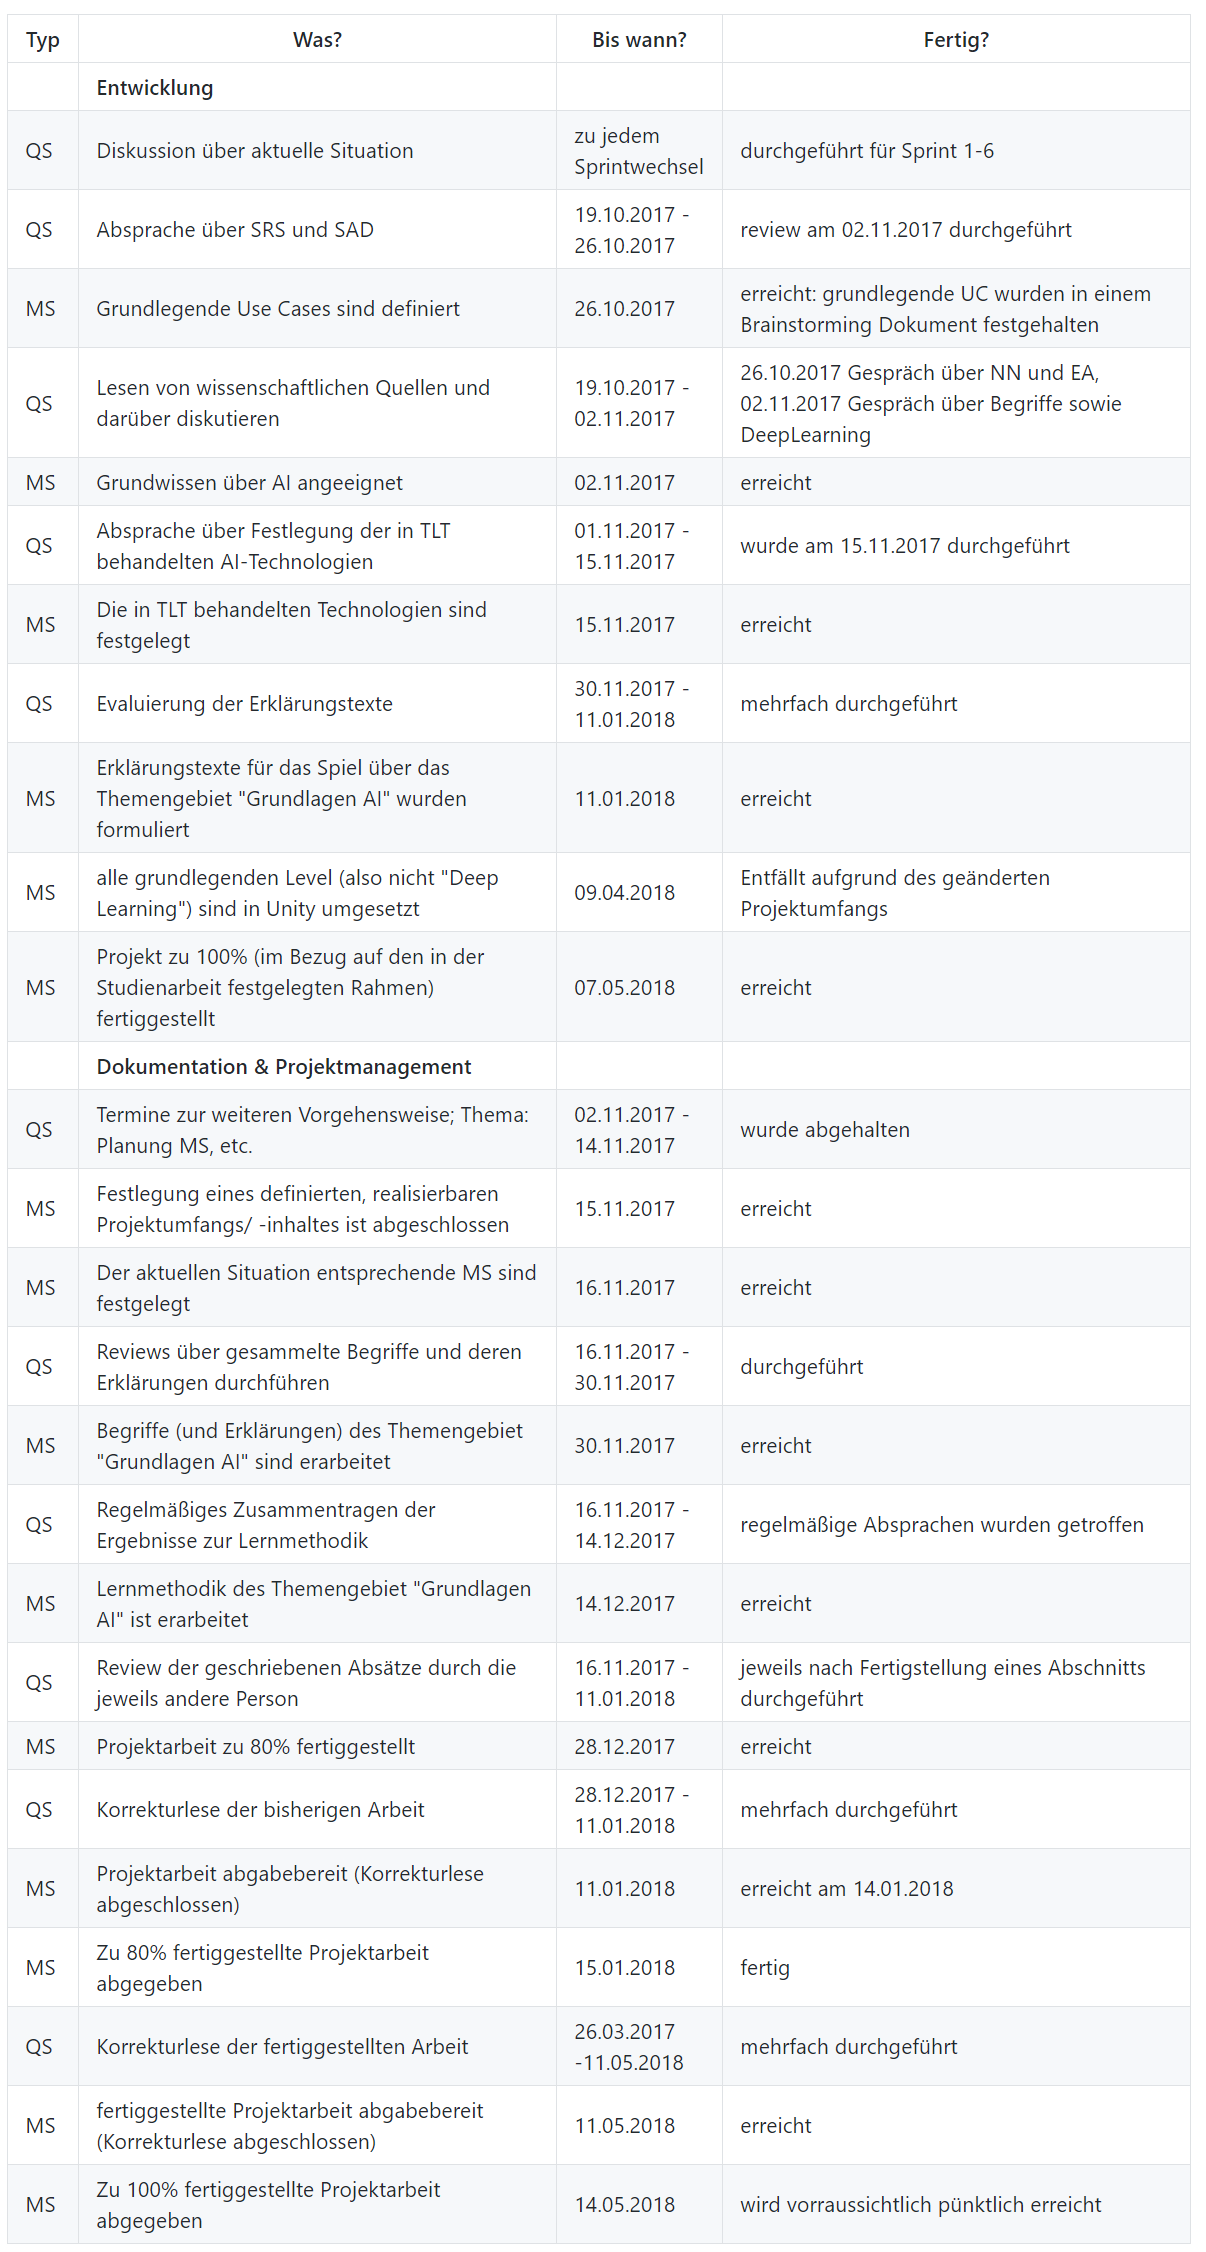
\includegraphics[scale=0.65]{bilder/QSMSS6.PNG}
\caption{QS und MS Analyse (Stand: 11.05.2018)}
\label{QSMSAnalyseBild}
\end{figure}

\begin{sidewaysfigure}[ht]
\centering
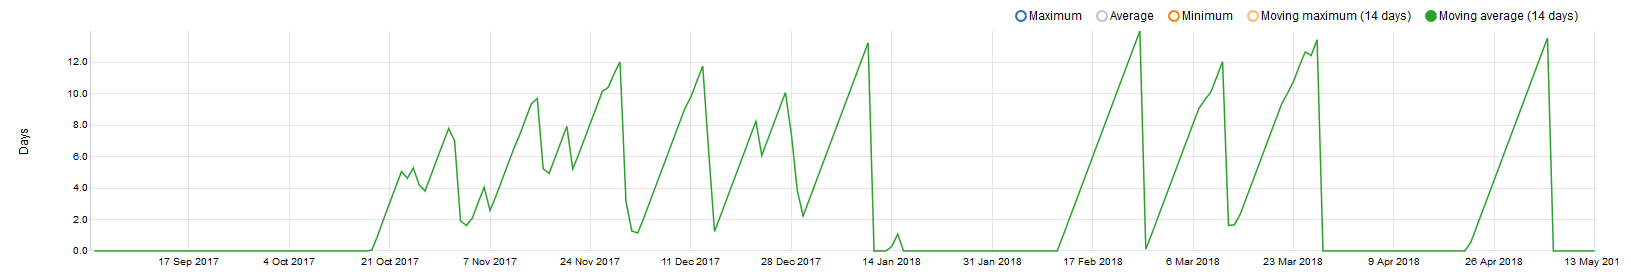
\includegraphics[scale=0.45]{bilder/ResoltutionTime.PNG}
\caption{Resolution Time Report (Stand: 13.05.2018)}
\label{RTimeReport}
\end{sidewaysfigure}

\begin{figure}[ht]
\centering
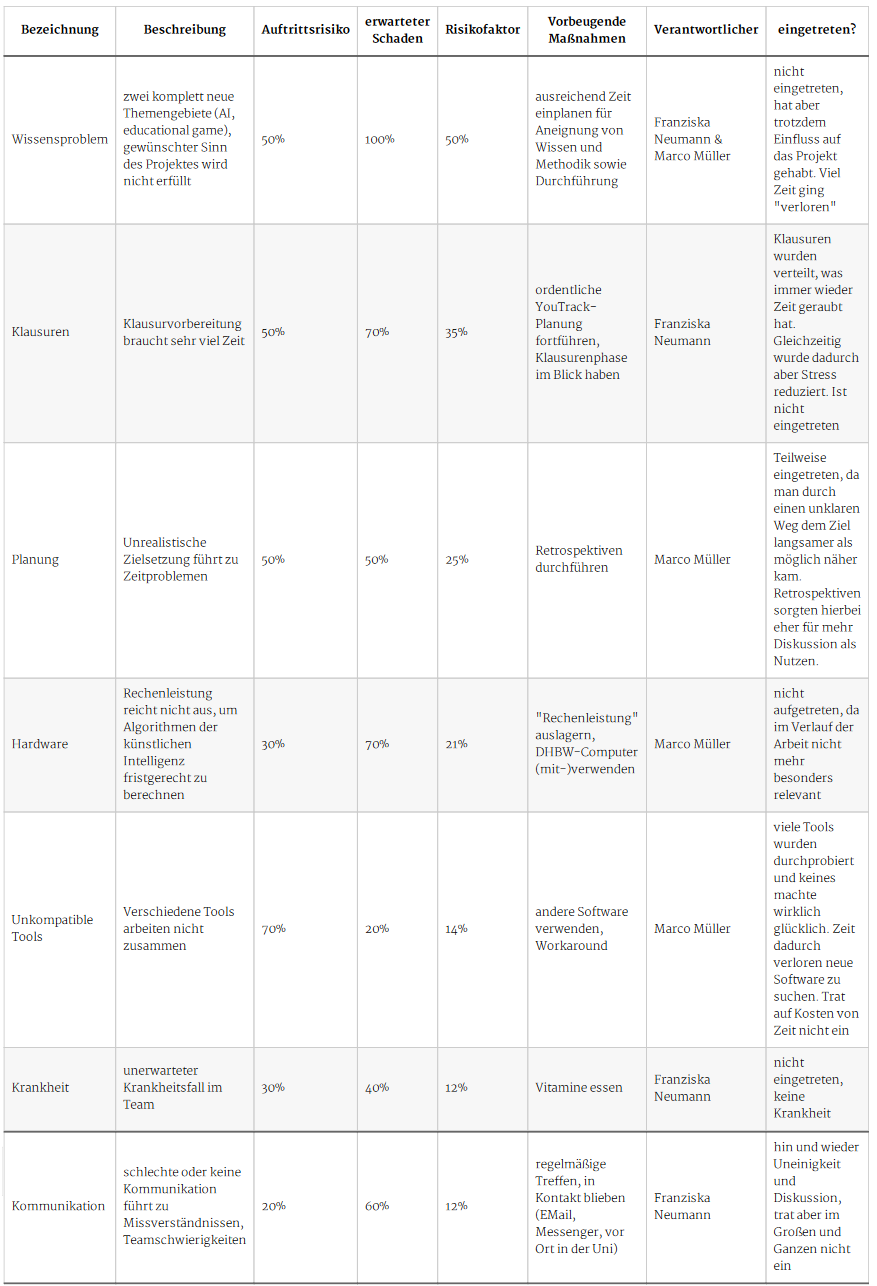
\includegraphics[scale=0.55]{bilder/RiskManagementTable.PNG}
\caption{Risk Management Table (Stand: 12.05.2018)}
\label{RiskManagementBild}
\end{figure}

\begin{sidewaysfigure}[ht]
\centering
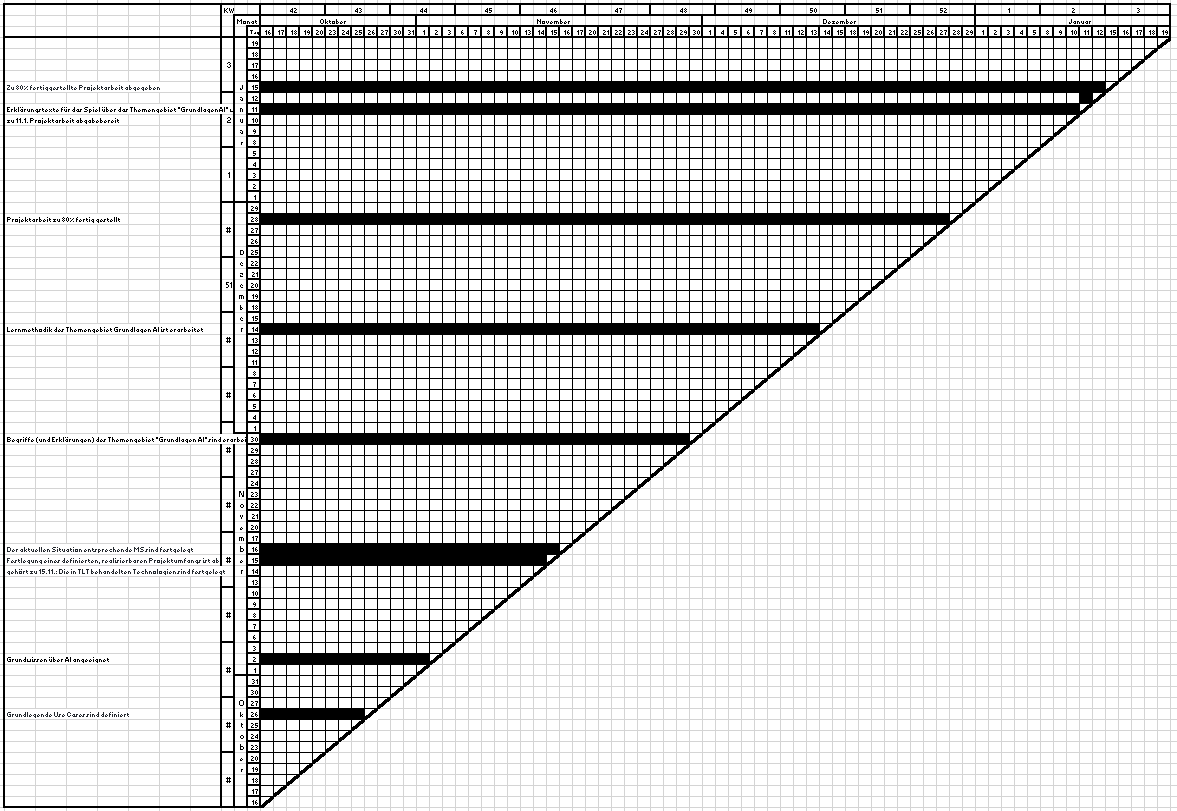
\includegraphics[scale=0.6]{bilder/MTA.PNG}
\caption{Meilenstein Trend Analyse (Stand: 14.01.2018)}
\label{MTA}
\end{sidewaysfigure}

\begin{sidewaysfigure}[ht]
\centering
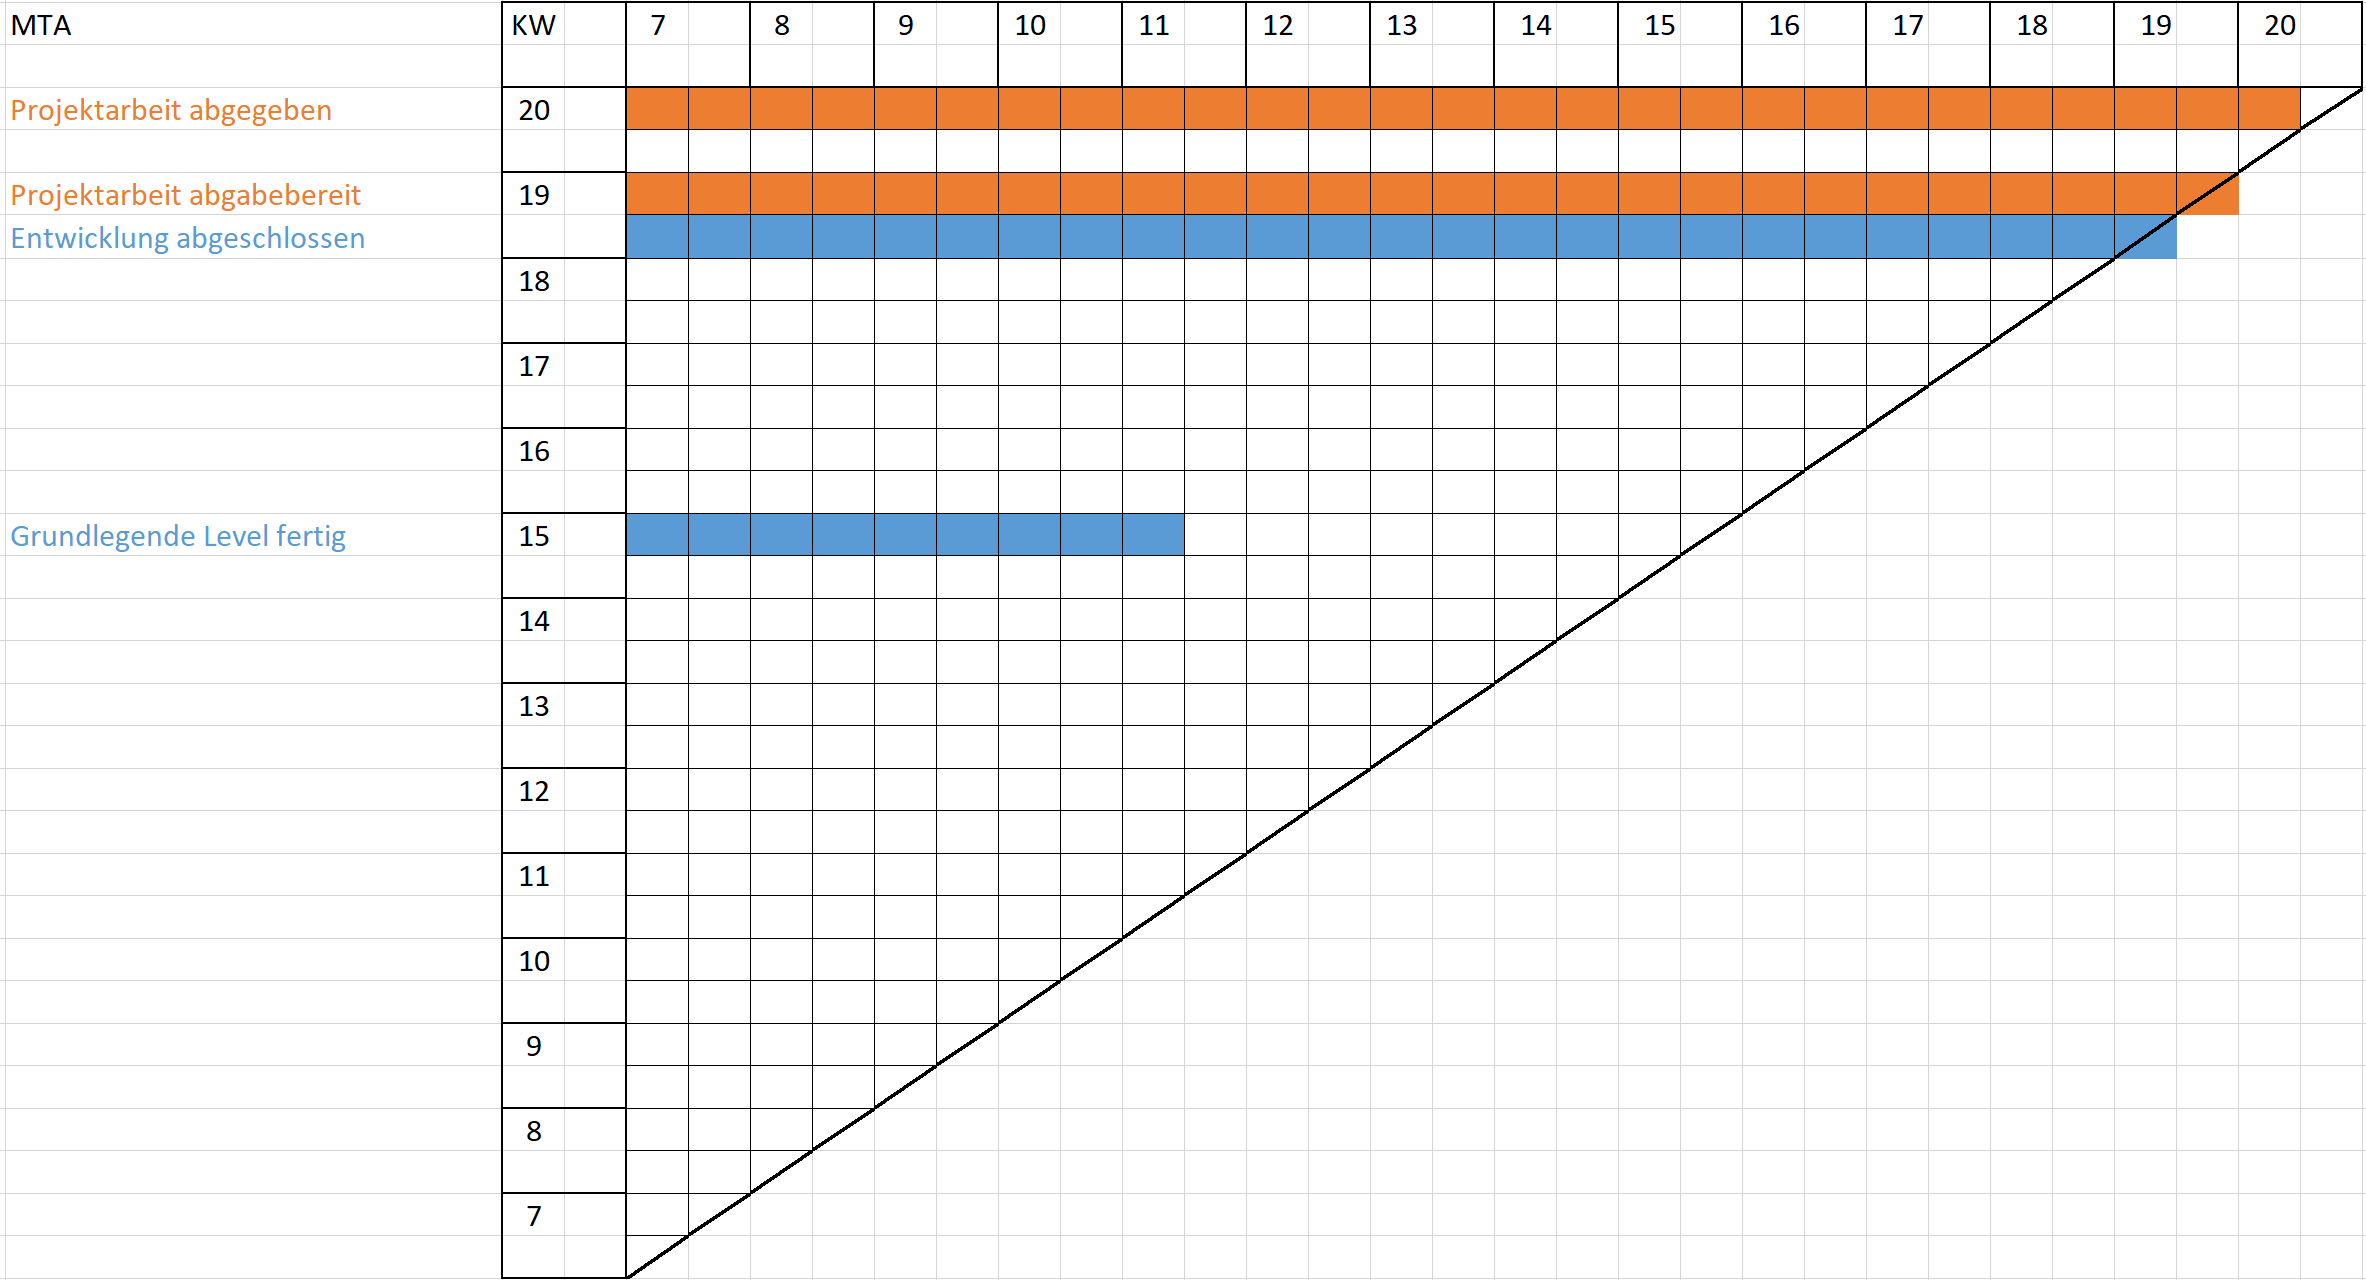
\includegraphics[scale=0.64]{bilder/MTAS6.PNG}
\caption{Meilenstein Trend Analyse (Stand: 11.05.2018)}
\label{MTA6}
\end{sidewaysfigure}
\end{appendix}

\end{document}